%% =====================================================================
%% main-llmxive.tex — content-extracted llmXive wrapper
%% =====================================================================
%% Generated by scripts/extract_paper_content.py. The original paper
%% body is preserved; the venue-specific preamble (class, bundled .cls
%% files, custom packages) is DISCARDED and replaced with the llmxive
%% house style + a shim block that no-ops any venue-specific macros the
%% body still references.
%% =====================================================================
\documentclass{llmxive}


%% ── Packages forwarded from original preamble ─────────────────
\usepackage{siunitx}
\usepackage{url}
\usepackage{multicol}
\usepackage{colortbl}
\usepackage{wrapfig}
\usepackage{makecell}
\usepackage{adjustbox}
\usepackage{fancyvrb}
\usepackage{soul}
\usepackage{float}
\usepackage{tikz}
\usepackage{fontawesome5}
\usepackage{longtable}
\usepackage{amsfonts}
\usepackage{graphicx}
\usepackage{subcaption}
\usepackage{xspace}
\usepackage{enumitem}
\usepackage{amsmath}
\usepackage{amssymb}
\usepackage{pifont}
\usepackage[ruled,linesnumbered]{algorithm2e}
\usepackage{listings}
\usepackage{tcolorbox}
\usepackage{multirow}
\usepackage{placeins}
\usepackage{hyphenat}
\usepackage{parskip}
\usepackage{lipsum}
\usepackage{etoolbox}
\usepackage[normalem]{ulem}
\usepackage{amsthm}
\usepackage{mathtools}
\usepackage{tabularx}
\usepackage[noabbrev,nameinlink]{cleveref}
\usepackage{natbib}

%% ── Shim layer (venue macros made into no-ops) ────────────────
\makeatletter
\providecommand{\TODO}[1]{}
\providecommand{\abscontent}{}
\providecommand{\absfont}{}
\providecommand{\acknowledgments}{\section*{Acknowledgments}}
\providecommand{\address}[1]{}
\providecommand{\affiliation}[1]{}
\providecommand{\aistatsfinalcopy}{}
\providecommand{\animategraphics}[5][]{\includegraphics[#1]{#3#4}}
\providecommand{\argmax}{\mathop{\mathrm{arg\,max}}}
\providecommand{\argmin}{\mathop{\mathrm{arg\,min}}}
\providecommand{\authornote}[1]{}
\providecommand{\authornotemark}[1][]{}
\providecommand{\authorrunning}[1]{}
\providecommand{\blfootnote}[1]{\footnote{#1}}
\providecommand{\bm}[1]{\boldsymbol{#1}}
\providecommand{\corresponding}{}
\providecommand{\correspondingauthor}[1]{}
\providecommand{\eg}{e.g.,\xspace}
\providecommand{\email}[1]{\href{mailto:#1}{#1}}
\providecommand{\equalcontribution}{}
\providecommand{\etal}{et al.\xspace}
\providecommand{\etc}{etc.\xspace}
\providecommand{\iclrfinalcopy}{}
\providecommand{\icmlfinalcopy}{}
\providecommand{\ie}{i.e.,\xspace}
\providecommand{\iid}{i.i.d.\xspace}
\providecommand{\institute}[1]{}
\providecommand{\keywords}[1]{\par\noindent\textbf{Keywords:} #1}
\providecommand{\neuripsfinalcopy}{}
\providecommand{\orcid}[1]{}
\providecommand{\tablecite}[1]{\cite{#1}}
\providecommand{\theabstract}{}
\providecommand{\titlerunning}[1]{}
\providecommand{\todo}[1]{}
\providecommand{\wrt}{w.r.t.\xspace}
\AtBeginDocument{\renewcommand{\and}{ \textperiodcentered\ }}
\makeatother

%% ── User-defined macros forwarded from original preamble ─────
\makeatletter
\providecommand{\red}[1]{{#1}}
\providecommand{\cmark}{\ding{51}}
\providecommand{\xmark}{\ding{55}}
\providecommand{\pmark}{\raisebox{0.1ex}{\scriptsize$\triangle$}}
\providecommand{\codepath}[1]{\texttt{\detokenize{#1}}}
\providecommand{\ourmethod}{\textsc{MobileForge}\xspace}
\providecommand{\mobilegym}{\textsc{MobileGym}\xspace}
\providecommand{\curriculum}{\textsc{MobileGym-Curriculum}\xspace}
\providecommand{\critic}{\textsc{MobileGym-Critic}\xspace}
\providecommand{\hifpo}{HiFPO\xspace}
\providecommand{\rise}[1]{#1}
\providecommand{\drop}[1]{#1}
\providecommand{\keyfinding}[1]{\noindent\textbf{#1}\quad}
\providecommand{\paperTable}{  \small
  \setlength{\tabcolsep}{4.5pt}  \renewcommand{\arraystretch}{1.12}}
\providecommand{\paperCompactTable}{  \footnotesize
  \setlength{\tabcolsep}{3.8pt}  \renewcommand{\arraystretch}{1.10}}
\providecommand{\paperDenseTable}{  \scriptsize
  \setlength{\tabcolsep}{3.2pt}  \renewcommand{\arraystretch}{1.08}}
\providecommand{\paperfigwide}{0.98\linewidth}
\providecommand{\paperfigmain}{0.94\linewidth}
\providecommand{\paperfigcompact}{0.80\linewidth}
\providecommand{\obsbox}[1]{  \begin{tcolorbox}[colframe=black!50, colback=forgeblue!45, boxrule=1pt, arc=2mm,
    top=4pt, bottom=4pt, left=6pt, right=6pt, boxsep=2pt, fontupper=\itshape]
    #1
  \end{tcolorbox}
}
\providecommand{\insight}[1]{  \par
  \refstepcounter{insight}  \addvspace{0.35em}  \noindent
  \begingroup
  \setlength{\fboxsep}{0pt}  \makebox[\linewidth][c]{    \colorbox{forgeblue}{      \parbox{0.97\linewidth}{        \vspace{0.35em}
        \hspace{0.65em}        \rule{1.4pt}{1.05em}        \hspace{0.55em}        \parbox[t]{0.88\linewidth}{          \textbf{\textsc{Insight}~\theinsight.}~#1        }        \vspace{0.35em}
      }    }  }  \endgroup
  \par\addvspace{0.35em}}
\providecommand{\resourceprojecticon}{\faGlobe}
\providecommand{\resourcegithubicon}{\faGithub}
\providecommand{\resourcehficon}{  \raisebox{0.3ex}{    \tikz[baseline=-0.5ex,scale=0.105]{      \fill[antblue] (0,0) circle (1);
      \fill[antblue] (-0.8,0.68) circle (0.34);
      \fill[antblue] (0.8,0.68) circle (0.34);
      \fill[white] (-0.34,0.22) circle (0.11);
      \fill[white] (0.34,0.22) circle (0.11);
      \draw[white,line width=0.12pt,line cap=round] (-0.36,-0.26) .. controls (0,-0.55) .. (0.36,-0.26);
    }  }}
\providecommand{\paperresourceicon}[4]{  #1\ \textbf{#2:}\ \href{#3}{{\ttfamily\fontsize{8}{9}\selectfont #4}}}
\providecommand{\titlefont}{\fontsize{14.4}{17}\selectfont}
\providecommand{\contributionlist}{\vspace{-2mm}}
\providecommand{\authorfootnotes}{{\scriptsize
\begin{tabular}{@{}l@{}}
\rule{47mm}{0.4pt}\\[-0.2ex]
$^*$Equal contribution.\quad $^\dagger$Project lead.\\[-0.2ex]
$^\S$Corresponding author.
\end{tabular}}}
\providecommand{\checkdatalist}{\begin{paperresources}
\paperresourceicon{\resourceprojecticon}{Project Page}{https://mobile-forge.github.io/}{mobile-forge.github.io}
\quad\quad
\paperresourceicon{\resourcehficon}{Datasets}{https://huggingface.co/collections/lgy0404/mobileforge-datasets}{lgy0404/mobileforge-datasets}\\
\paperresourceicon{\resourcegithubicon}{Code}{https://github.com/kwai/MobileForge}{github.com/kwai/MobileForge}
\quad\quad
\paperresourceicon{\resourcehficon}{Models}{https://huggingface.co/collections/lgy0404/mobileforge-models}{lgy0404/mobileforge-models}
\end{paperresources}}
\@ifundefined{paperresources}{\newenvironment{paperresources}{\par\noindent\begin{minipage}{0.92\textwidth}
    \centering\footnotesize\sffamily
    \setlength{\parindent}{0pt}\setlength{\parskip}{2pt}}{\end{minipage}\par\vspace{1.7mm}}}{}
\newcolumntype{L}[1]{>{\raggedright\arraybackslash}p{#1}}
\newcolumntype{C}[1]{>{\centering\arraybackslash}p{#1}}
\newcolumntype{R}[1]{>{\raggedleft\arraybackslash}p{#1}}
\usetikzlibrary{arrows.meta,positioning,fit}
\definecolor{forgeblue}{HTML}{E3F2FD}
\definecolor{forgelight}{HTML}{F5F7FA}
\definecolor{forgepurple}{HTML}{7E57C2}
\definecolor{forgegreen}{HTML}{43A047}
\definecolor{forgered}{HTML}{FB8C00}
\definecolor{forgegray}{HTML}{E0E0E0}
\definecolor{forgeprimary}{HTML}{1565C0}
\definecolor{forgeprimarydark}{HTML}{0D47A1}
\definecolor{forgecyan}{HTML}{00ACC1}
\definecolor{oursrowcolor}{HTML}{E3F2FD}
\definecolor{baselinerowcolor}{HTML}{F5F7FA}
\definecolor{alibabaorange}{HTML}{FF6A00}
\definecolor{lightred}{RGB}{255, 182, 193}
\definecolor{lightgreen}{RGB}{144, 238, 144}
\definecolor{lightblue}{RGB}{173, 216, 230}
\definecolor{lightergray}{gray}{0.90}
\definecolor{metabg}{HTML}{FFF4EB}
\definecolor{ourg}{rgb}{0.23,0.49,0.14}
\definecolor{ourb}{rgb}{0.13,0.37,0.60}
\definecolor{ourp}{rgb}{0.44,0.18,0.63}
\definecolor{ouro}{rgb}{0.87,0.69,0.23}
\definecolor{ouro2}{rgb}{1,0.753,0}
\definecolor{upcolor}{rgb}{0.21,0.49,0.74}
\definecolor{our-yellow}{rgb}{221,175,57}
\definecolor{our-blue}{rgb}{29,113,168}
\tcbuselibrary{breakable,listings}
\newtcolorbox[auto counter]{promptbox}[1][]{
    top=15pt,
    bottom=15pt,
    left=20pt,
    right=20pt,
    colback=gray!5,
    colframe=black,
    fonttitle=\bfseries,
    coltitle=white,
    title=Prompt~\thetcbcounter: #1,
    breakable,
    fontupper=\ttfamily\small,
}
\newtcolorbox{insightline}{
    blanker,
    breakable,
    left=4.5mm, right=4.5mm, top=1.5mm, bottom=1.5mm,
    borderline west={2pt}{0pt}{antblue},
    colback=gray!5, 
    fontupper=\itshape
}
\newtcolorbox{insightbox}{
  enhanced,
  breakable,
  colback=metabg,
  colframe=black!70,
  boxrule=0.7pt,
  arc=2.2mm,
  left=8pt,right=8pt,top=6pt,bottom=6pt, 
  title=\textbf{Key Insights in Reward Design},
  colbacktitle=black!85,
  coltitle=white,
  fonttitle=\bfseries\ttfamily\footnotesize,
  attach boxed title to top left={xshift=5mm,yshift=-2mm},
  boxed title style={
    boxrule=0pt,
    arc=1.2mm,
    left=2.2mm,right=2.2mm,top=1mm,bottom=1mm
  }
}
\newtcolorbox{theorybox}[1][]{  enhanced, breakable,
  colback=metabg,   
  colframe=metabg,  
  boxrule=0pt,            
  arc=2mm,                
  left=8pt,right=8pt,top=6pt,bottom=6pt, 
  before skip=8pt, after skip=8pt,
  #1
}
\newtcolorbox{systempromptbox}{
  enhanced,
  breakable,
  colback=gray!8,
  colframe=black!70,
  boxrule=0.7pt,
  arc=2.2mm,
  left=5mm,right=5mm,top=4mm,bottom=4mm,
  title=\texttt{SYSTEM\_PROMPT},
  colbacktitle=black!85,
  coltitle=white,
  fonttitle=\bfseries\ttfamily\footnotesize,
  attach boxed title to top left={xshift=5mm,yshift=-2mm},
  boxed title style={
    boxrule=0pt,
    arc=1.2mm,
    left=2.2mm,right=2.2mm,top=1mm,bottom=1mm
  }
}
\makeatother

%% ── llmXive paper metadata ──────────────────────────────────
\title{MobileForge: Annotation-Free Adaptation for Mobile GUI Agents with Hierarchical Feedback-Guided Policy Optimization}
\author{Guangyi Liu \and Pengxiang Zhao \and Gao Wu \and Yiwen Yin \and Mading Li \and Liang Liu \and Congxiao Liu \and Zhang Qi \and Mengyan Wang \and Liang Guo \and Yong Liu}
\paperid{arXiv:2606.19930}
\paperstatus{Preprint}

\begin{document}
\maketitle
\begin{abstract}
MLLM-based mobile GUI agents have made substantial progress in UI understanding and action execution, but adapting them to real target apps remains costly because mobile apps are numerous, frequently updated, and hard to cover with human-written tasks, demonstrations, or reward labels. Existing annotation-free GUI learning reduces manual supervision, yet lacks a unified substrate connecting target-app exploration, curriculum mining, rollout execution, and feedback, while policy optimization often relies on isolated rollouts and coarse rewards that are hard to convert into reliable improvement signals. We present \textbf{\ourmethod}, an annotation-free adaptation system for mobile GUI agents. \ourmethod consists of \textbf{\mobilegym}, which grounds task generation and rollout evaluation in real mobile app interaction, and \textbf{\underline{Hi}}erarchical \textbf{\underline{F}}eedback-Guided \textbf{\underline{P}}olicy \textbf{\underline{O}}ptimization (\textbf{\hifpo}), which turns trajectory outcomes, step-level process feedback, and corrective hints into hint-contextualized step-level GRPO updates. Using only automatically generated annotation-free adaptation data, \ourmethod adapts \llmname{Qwen3-VL-8B} to 67.2\% Pass@3 on AndroidWorld, close to the closed-data GUI-specialized \llmname{GUI-Owl-1.5-8B} base model at 69.0\%. The MobileForge-adapted \llmname{ForgeOwl-8B} further reaches 77.6\% Pass@3 on AndroidWorld and 41.0\% success on the out-of-domain MobileWorld GUI-only split, establishing the strongest open-data mobile GUI agent in our evaluation. Code, data, and trained models will be released at \url{https://mobile-forge.github.io/}.
\end{abstract}
\enlargethispage{6\baselineskip}
\begingroup
\vspace*{-2.0em}
\captionsetup{font=footnotesize}
\noindent\makebox[\textwidth][c]{%
\begin{minipage}{0.99\textwidth}
    \centering
    
    \vspace{-0.5em}
    \captionof{figure}{\textbf{Main performance of \ourmethod.}
    \ourmethod scales with generated AndroidWorld tasks, improves in-domain AndroidWorld performance, and transfers to the MobileWorld GUI-only split.}
    \label{fig:main-performance}
\end{minipage}}
\vspace{-0.8em}
\endgroup



\begin{figure}[t]
    \centering
    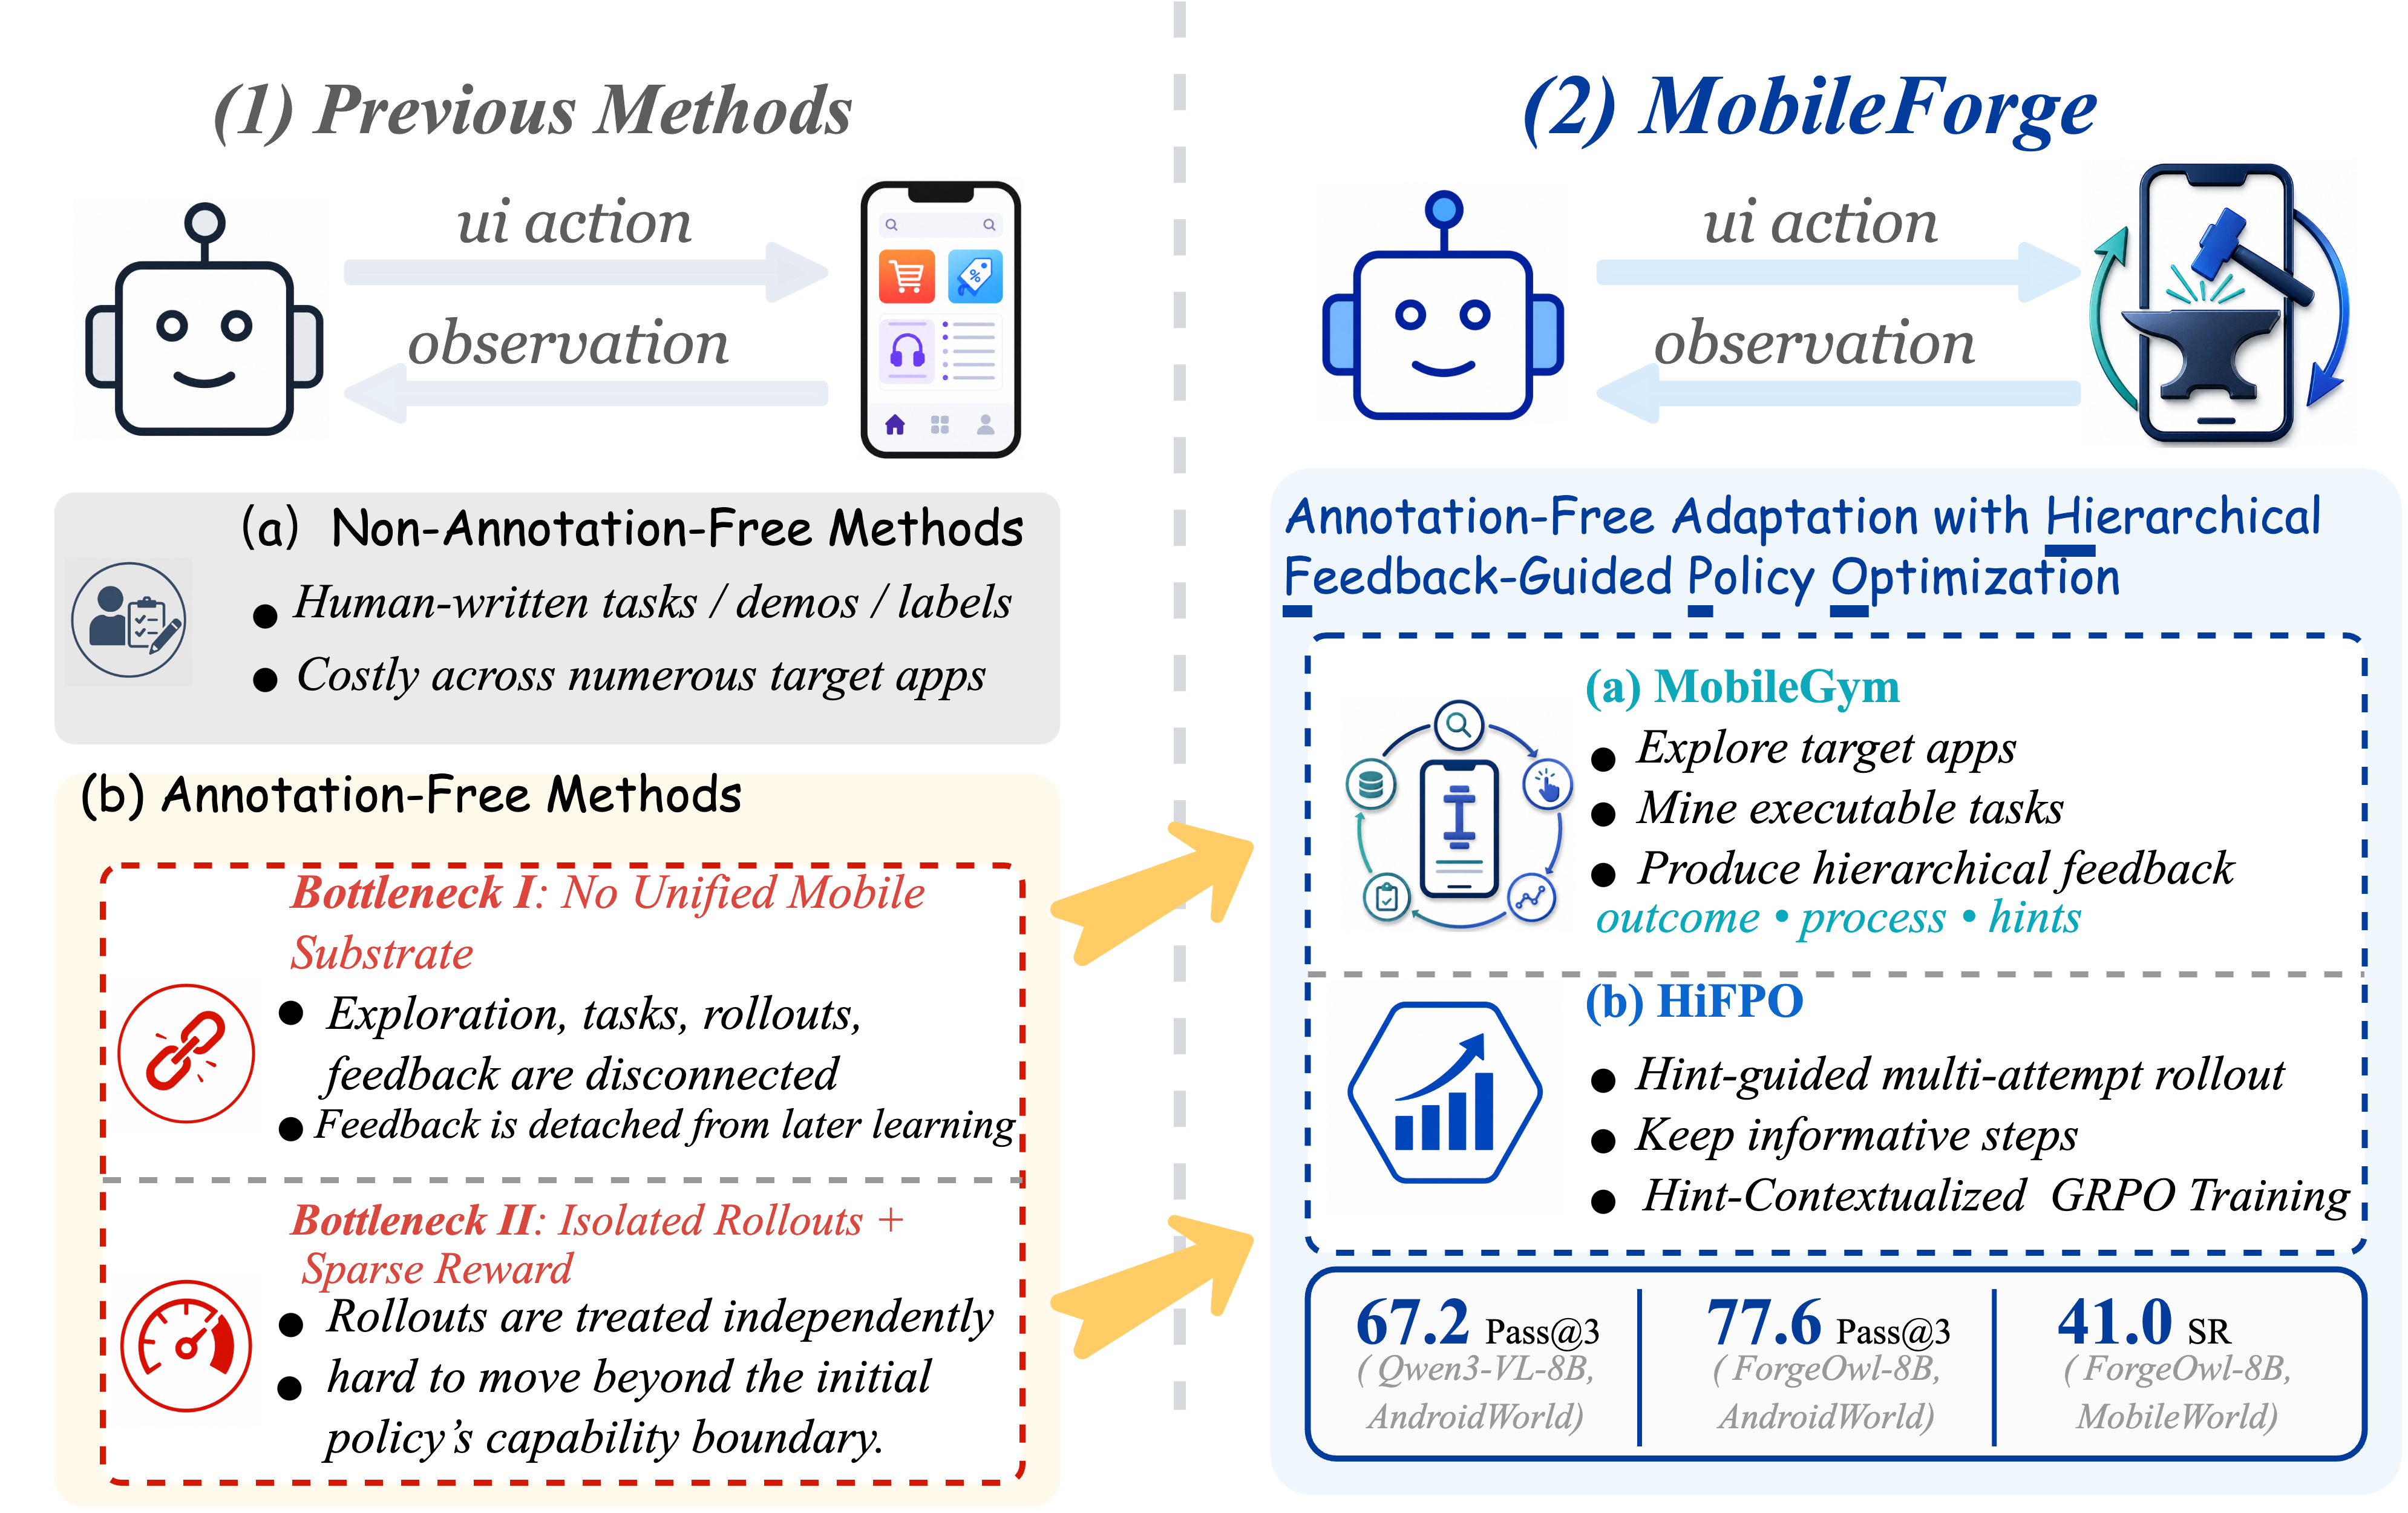
\includegraphics[width=0.99\linewidth]{images/teaser/mobileforge-teaser-latex.png}
    \vspace{-2mm}
    \caption{\textbf{Motivation and overview of \ourmethod.} Existing annotation-free GUI learning lacks a unified adaptation substrate and relies on isolated sparse-reward rollouts. \ourmethod combines \mobilegym for target-app exploration, task mining, and hierarchical feedback with \hifpo for hint-guided rollout, step selection, and hint-contextualized GRPO.}
    \label{fig:mobileforge-teaser}
\end{figure}

\section{Introduction}
\label{sec:introduction}

MLLM-based mobile GUI agents have made substantial progress in UI understanding and action execution~\cite{gao2026ui,zhou2025mai,hong2024cogagent,xu2026mobile,liu2025llm}. However, real deployment requires adaptation beyond fixed benchmarks. Mobile apps are numerous and fast-changing, making human-written tasks, expert demonstrations, and manual reward labels costly and quickly stale \citep{zhang2025tongui,wang2025mobilea3gent,sun2025genesis,yang2025zerogui}. This motivates annotation-free adaptation, where an agent discovers target-app functions, attempts executable tasks, evaluates behavior, and improves from the experience.

Recent annotation-free GUI agent work has reduced human supervision. TongUI mines supervision from web tutorials \citep{zhang2025tongui}, MobileA3gent uses decentralized user-phone trajectories \citep{wang2025mobilea3gent}, OS-Genesis synthesizes GUI tasks through reverse task construction \citep{sun2025genesis}, and GUI-explorer mines transition-aware interaction knowledge through autonomous exploration \citep{xie2025gui}. ZeroGUI and MobileGUI-RL study automatic reward estimation and online reinforcement learning \citep{yang2025zerogui,shi2025mobilegui}, while SEAgent, ACuRL, and UI-Oceanus explore self-evolving, continual, or synthetic-environment scaling for broader computer-use agents \citep{sun2025seagent,xue2026acurl,wu2026uioceanus}. Appendix~\ref{sec:related} provides a taxonomy.

Despite these advances, two bottlenecks still limit mobile target-app adaptation. \textbf{(I)} Existing methods \textbf{lack a unified mobile substrate} connecting target-app exploration, curriculum mining, rollout execution, and feedback, so generated tasks may be weakly grounded and evaluator feedback may remain detached from policy learning. \textbf{(II)} Policy optimization often treats rollouts as \textbf{isolated experiences with sparse reward}; even with step-level assessment, current loops rarely combine outcomes, process feedback, and corrective hints to accumulate reusable experience beyond the initial policy's capability boundary. Figure~\ref{fig:mobileforge-teaser} illustrates these bottlenecks and our solution.

\obsbox{\textbf{Research question.} Can we build an annotation-free adaptation system for mobile GUI agents that grounds tasks in target-app interaction, generates fine-grained feedback, and converts self-collected experience into policy-improvement signals without human-written tasks, demonstrations, or reward labels?}

We introduce \textbf{\ourmethod}, an annotation-free adaptation system with hierarchical feedback-guided policy optimization. \textbf{\emph{(i)}} \textbf{\mobilegym} is the interaction and evaluation substrate: \curriculum mines executable tasks from target-app traces, while \critic evaluates rollouts with outcome feedback, step-level feedback, and corrective hints. \textbf{\emph{(ii)}} \textbf{\underline{Hi}}erarchical \textbf{\underline{F}}eedback-Guided \textbf{\underline{P}}olicy \textbf{\underline{O}}ptimization (\textbf{\hifpo}) schedules hint-guided attempts, filters tasks and steps with hierarchical feedback, and trains the policy with hint-contextualized step-level GRPO.

We evaluate \ourmethod on AndroidWorld \citep{rawles2024androidworld} as the in-domain setting and MobileWorld GUI-only \citep{kong2026mobileworld} as the out-of-domain setting, with no MobileWorld rollout used for training. As shown in Figure~\ref{fig:main-performance}, annotation-free adaptation narrows the gap to closed-data GUI-specialized agents: \llmname{Qwen3-VL-8B}~\citep{bai2025qwen3} reaches 67.2\% Pass@3 on AndroidWorld using generated adaptation data, close to the \llmname{GUI-Owl-1.5-8B}~\citep{xu2026mobile} base model at 69.0\%. \ourmethod further improves GUI-Owl, yielding \llmname{ForgeOwl-8B} with 77.6\% Pass@3 on AndroidWorld and 41.0\% success on MobileWorld GUI-only, the strongest open-data mobile GUI agent in our evaluation.

\paragraph{Contributions.}
\textbf{(1)} We identify two bottlenecks in annotation-free mobile GUI adaptation: the lack of a unified target-app interaction and evaluation substrate, and isolated rollouts with coarse feedback for policy optimization.
\textbf{(2)} We propose \textbf{\mobilegym}, which grounds exploration, curriculum mining, rollout execution, and hierarchical evaluation in real mobile app interaction.
\textbf{(3)} We propose \textbf{\underline{Hi}}erarchical \textbf{\underline{F}}eedback-Guided \textbf{\underline{P}}olicy \textbf{\underline{O}}ptimization (\textbf{\hifpo}), which transforms multi-attempt feedback and corrective hints into hint-contextualized step-level GRPO updates.
\textbf{(4)} We show that \ourmethod improves generalist and GUI-specialized agents, transfers from AndroidWorld to MobileWorld GUI-only, and yields \llmname{ForgeOwl-8B}, the strongest open-data mobile GUI agent in our evaluation.

\section{\ourmethod}
\label{sec:method}

\ourmethod is an annotation-free adaptation system for mobile GUI agents. We consider a setting where target mobile apps and an initial GUI policy are available, but no human-written tasks, expert demonstrations, or reward labels are provided for those apps. The system therefore needs to ground task generation in real target-app interaction, collect rollout experience, evaluate its own behavior, and update the policy from the resulting feedback. Figure~\ref{fig:mobileforge-overview} illustrates the overall loop.

\begin{figure}[!htbp]
    \centering
    \includegraphics[width=0.8\linewidth]{images/mobileforge-overview/mobileforge-overview.drawio.png}
    \caption{\textbf{Overview of \ourmethod.}
}
    \label{fig:mobileforge-overview}
\end{figure}


\subsection{Problem Setup}

We model mobile GUI control as sequential decision making over observed GUI states. Let $x\in\mathcal{T}$ denote a generated task. For attempt $k$ on task $x$ and step $t$, the policy receives a \emph{decision state}
\begin{equation}
\label{eq:decision-state}
    s_k^{(t)}=(x,I_k^{(t)},\mathcal{H}_k^{(t)},\eta_{<k}),
\end{equation}
where $I_k^{(t)}$ is the screenshot observation, $\mathcal{H}_k^{(t)}$ is the interaction history, and $\eta_{<k}$ is the corrective hint context accumulated from earlier attempts of the same task. The policy emits a structured GUI action
\begin{equation}
\label{eq:gui-action}
    a_k^{(t)}=(\alpha_k^{(t)},\psi_k^{(t)})
    \sim \pi_\theta(\cdot\mid s_k^{(t)}),
\end{equation}
where $\alpha$ is the action type, such as tap, swipe, type, wait, terminate, answer, or system navigation, and $\psi$ contains the corresponding arguments, such as coordinates, direction, text, or termination status. A rollout attempt is the sequence
\begin{equation}
\label{eq:trajectory}
    \tau_k=(s_k^{(1)},a_k^{(1)},\ldots,s_k^{(T_k)},a_k^{(T_k)}).
\end{equation}

The environment does not provide a dense scalar reward during rollout. Instead, \critic evaluates a completed attempt and returns labels and hints. We reserve $R$ for the numeric action reward used later by GRPO, and use $z$ and $\ell$ for evaluator feedback labels. This distinction is important: \ourmethod first converts attempts into structured feedback, then converts selected steps into policy-optimization rewards.

\ourmethod contains the two coupled components introduced in Section~\ref{sec:introduction}. \mobilegym is the interaction and evaluation substrate: it explores target apps, mines executable tasks, executes rollouts, and evaluates completed rollouts through a hierarchical critic. \hifpo is the adaptation algorithm: it schedules hint-guided attempts over the MobileGym curriculum, filters tasks and steps with hierarchical feedback, and updates the policy with hint-contextualized step-level GRPO. The loop can be summarized as:
\begin{equation}
\label{eq:mobileforge-loop}
\begin{aligned}
\mathcal{Z} &\leftarrow \operatorname{Explore}(\mathcal{E}),\\
\mathcal{T} &\leftarrow \operatorname{Curriculum}(\mathcal{Z}),\\
\{\tau_k\}_{k=1}^{K} &\leftarrow
\operatorname{Rollout}(\pi_\theta,x,\eta_{<k}),\quad \forall x\in\mathcal{T},\\
\mathcal{F}_{k} &\leftarrow \operatorname{Critic}(x,\tau_k),\\
\mathcal{D} &\leftarrow \operatorname{HiFPO}(\mathcal{T},\tau,\mathcal{F}),\\
\theta' &\leftarrow \operatorname{GRPO}(\theta,\mathcal{D}).
\end{aligned}
\end{equation}
Here $\mathcal{Z}$ is exploration evidence, $\mathcal{T}$ is the generated curriculum, $\mathcal{F}_{k}$ is hierarchical feedback for attempt $\tau_k$ on task $x$, and $\mathcal{D}$ is the filtered step-level training set. Appendix~\ref{sec:appendix_method_details} provides the full notation table (Table~\ref{tab:method_notation}) and a compact pseudocode summary of the adaptation loop (Algorithm~\ref{alg:mobileforge}).

\subsection{\mobilegym: Building an Adaptation Substrate}
\label{sec:mobilegym}

\mobilegym answers the question: \emph{where do executable tasks and rollout feedback come from without human-written tasks, demonstrations, or reward labels?} It turns target-app interaction into three artifacts needed by policy learning: exploration evidence, executable tasks, and hierarchical evaluation of completed rollouts. Figure~\ref{fig:mobilegym} summarizes this substrate. Importantly, \mobilegym is the substrate and evaluator; the strategy for running multiple attempts and reusing hints belongs to \hifpo.

\begin{figure}[!htbp]
    \centering
    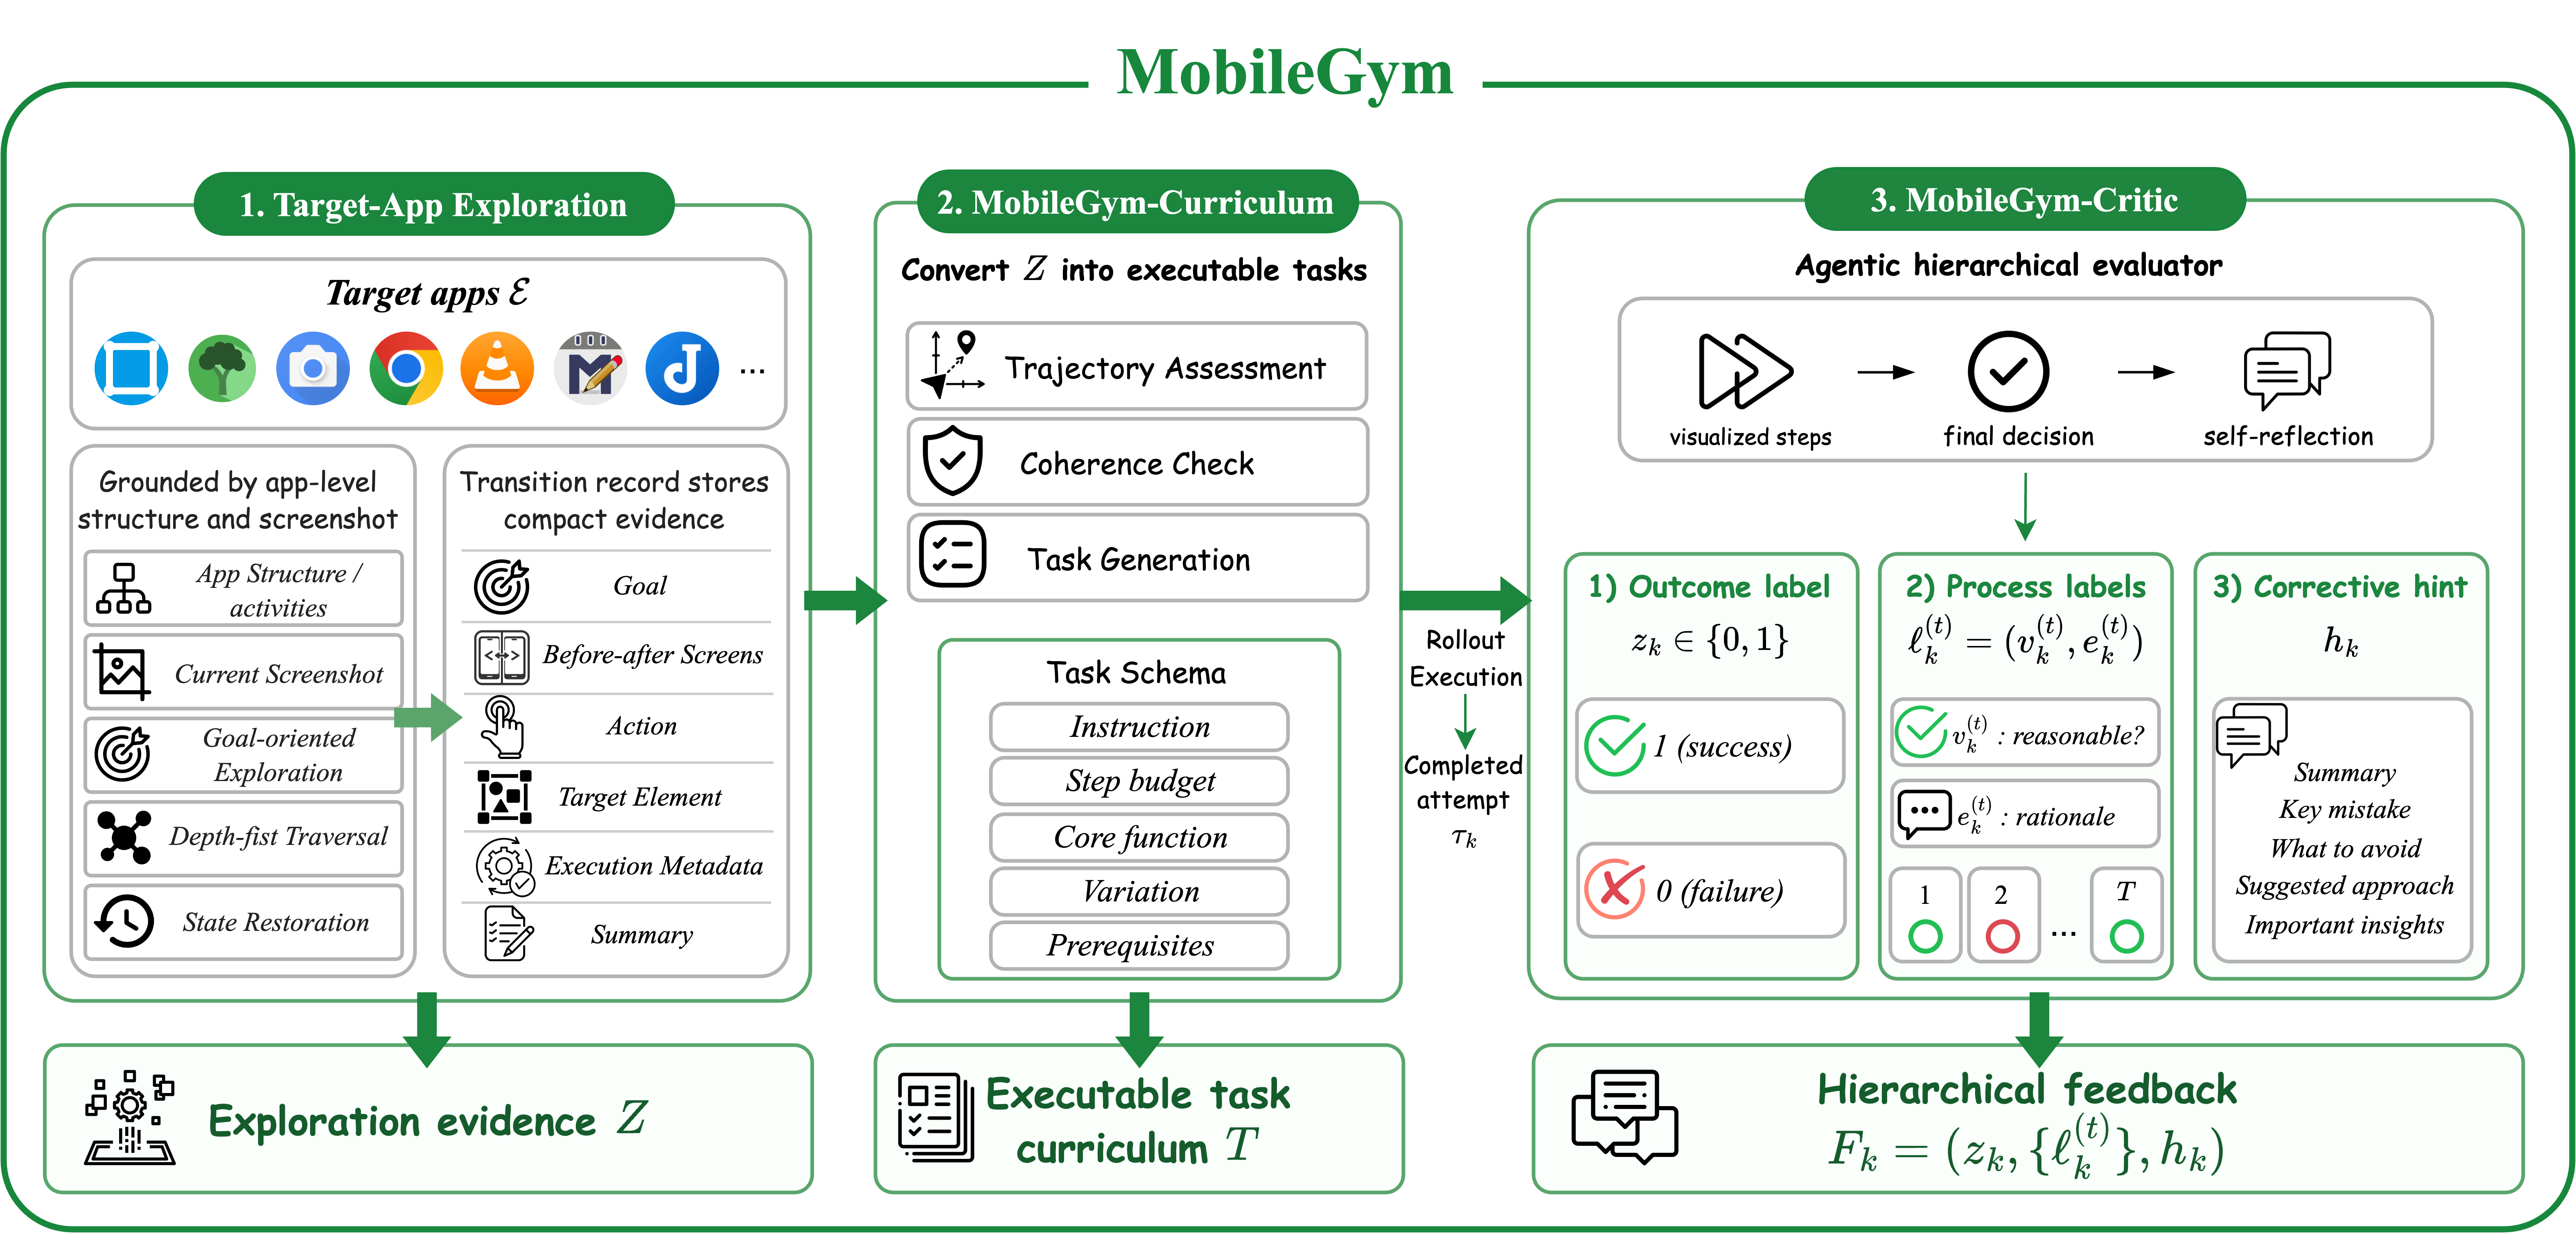
\includegraphics[width=\paperfigmain]{images/mobilegym/mobilegym.drawio.png}
    \caption{\textbf{\mobilegym as the annotation-free adaptation substrate.}
    \mobilegym grounds adaptation in real target-app interaction: it explores reachable GUI states, mines trajectory-grounded tasks through \curriculum, and evaluates completed attempts with \critic to produce trajectory-level outcomes, step-level process feedback, and corrective hints.}
    \label{fig:mobilegym}
\end{figure}


\subsubsection{Target-App Exploration}

\ourmethod first explores each target app directly. We use a function-aware exploration strategy inspired by GUI-explorer \citep{xie2025gui}: app-level structural anchors, such as activities declared in the APK, are combined with the current screenshot to generate goal-oriented exploration tasks. The explorer then pursues these goals with depth-first traversal, restoring parent states when branching and recording the resulting interactions. Exploration is not treated as expert demonstration. Its role is to discover reachable screens, UI affordances, and app functions, giving the system an app-grounded basis for task generation instead of relying on generic assumptions about what an app might support. Appendix~\ref{sec:exploration_details} provides more details.

Each explored transition records the before/after screens, executed action, target element, and a short natural-language summary. These transition records form $\mathcal{Z}$, the evidence pool used by the curriculum stage.

\subsubsection{\curriculum}
\label{sec:curriculum}

\curriculum converts exploration evidence into executable tasks. For each explored trajectory, it checks whether the observed behavior is coherent and whether the intended function appears completed. It then generates task variants grounded in the same reachable app states and functions.

We write a generated task as
\begin{equation}
    x=(\iota,B,c,v,p),
\end{equation}
where $\iota$ is the instruction, $B$ is an estimated step budget, $c$ is the core functionality, $v$ is the variation type, and $p$ describes prerequisites. The schema is lightweight by design; the key property is that each task is grounded in observed app behavior.
The curriculum prompt jointly evaluates the explored trajectory and asks for self-contained task variants; Appendix~\ref{sec:curriculum_prompt} shows the core template.

\subsubsection{Hierarchical Rollout Evaluation}
\label{sec:evaluation}

Given a completed rollout attempt $\tau_k$ for task $x$, \critic produces hierarchical feedback:
\begin{equation}
\label{eq:feedback-object}
    \mathcal{F}_{k}
    =\left(z_{k},\{\ell_k^{(t)}\}_{t=1}^{T_k},h_k\right).
\end{equation}
\critic is implemented as an agentic hierarchical evaluator rather than a learned reward model. It first converts the raw execution log into visual action traces: each step is rendered as an action-centered screenshot, and a VLM describes the performed action and task-relevant screen evidence. A final decision model then receives the task, raw action logs, step descriptions, and a stitched view of the last screenshots, and returns a structured JSON verdict. Appendix~\ref{sec:critic_prompts} shows the core prompts.

The trajectory outcome label $z_k\in\{0,1\}$ is the final decision field: $z_k=1$ means that the attempt completed the task, while $z_k=0$ means failure. The evaluator also reports task feasibility, a failure step when applicable, and a natural-language reason. The step-level process label $\ell_k^{(t)}$ summarizes the local quality of step $t$. We represent it as
\begin{equation}
\label{eq:process-label}
    \ell_k^{(t)}=(v_k^{(t)},e_k^{(t)}),
\end{equation}
where $v_k^{(t)}\in\{0,1\}$ is derived from the evaluator's reasonable/unreasonable step tag, and $e_k^{(t)}$ is the step-level rationale. The corrective hint $h_k$ is generated when an attempt fails or contains unreasonable steps; it summarizes key mistakes, what to avoid, suggested alternatives, and important task insights. \hifpo decides how to reuse this hint in later rollouts and training prompts.

This hierarchy separates three roles that are often collapsed into one signal. Outcome labels decide whether a task is solved. Process labels identify useful local decisions inside both successful and failed attempts. Hints carry reusable failure information across attempts and into training prompts.

\begin{figure}[!htbp]
    \centering
    \includegraphics[width=\paperfigmain]{images/hifpo/hifpo.drawio.png}
    \caption{\textbf{\hifpo converts hierarchical feedback into policy updates.}
    \hifpo performs hint-guided multi-attempt rollout, removes mastered all-success tasks, retains difficult and partially solved tasks, extracts reasonable local steps from hierarchical feedback, and trains the policy with hint-contextualized step-level GRPO.}
    \label{fig:hifpo}
\end{figure}


\subsection{\hifpo: Feedback-Guided Policy Optimization}
\label{sec:optimization}

\hifpo answers the question: \emph{how can self-collected rollout experience become effective policy-improvement signals instead of isolated attempts with sparse feedback?} Figure~\ref{fig:hifpo} shows the pipeline. \hifpo first runs hint-guided multi-attempt rollouts over the \mobilegym curriculum, calls \critic to evaluate completed attempts, removes tasks already mastered by the current policy, selects informative attempts and reasonable local steps, and finally trains with hint-contextualized step-level GRPO.

\subsubsection{Hint-Guided Multi-Attempt Rollout}

For each generated task, \hifpo runs $K$ attempts. Attempts of the same task are serialized so that feedback from earlier attempts can condition later attempts, while different tasks can be collected in parallel. Before attempt $k$, \hifpo builds a hint context $\eta_{<k}$ from corrective hints produced by \critic on attempts $1,\ldots,k-1$:
\begin{equation}
\label{eq:hint-context}
    \eta_{<k}=\operatorname{Aggregate}(h_1,\ldots,h_{k-1}).
\end{equation}
The next attempt is sampled as
\begin{equation}
\label{eq:hifpo-rollout}
    \tau_k\sim \operatorname{Rollout}(\pi_\theta,x,\eta_{<k}).
\end{equation}
\mobilegym provides the interaction substrate and \critic evaluation for each completed attempt; \hifpo controls the repeated-attempt protocol and decides how hints are accumulated and reused. This separation keeps \mobilegym focused on target-app interaction and hierarchical evaluation, while \hifpo defines the feedback-guided optimization behavior.
Figure~\ref{fig:case-add-hint} illustrates how corrective hints from earlier attempts are reused to guide later attempts.
\begin{figure}[t]
    \centering
    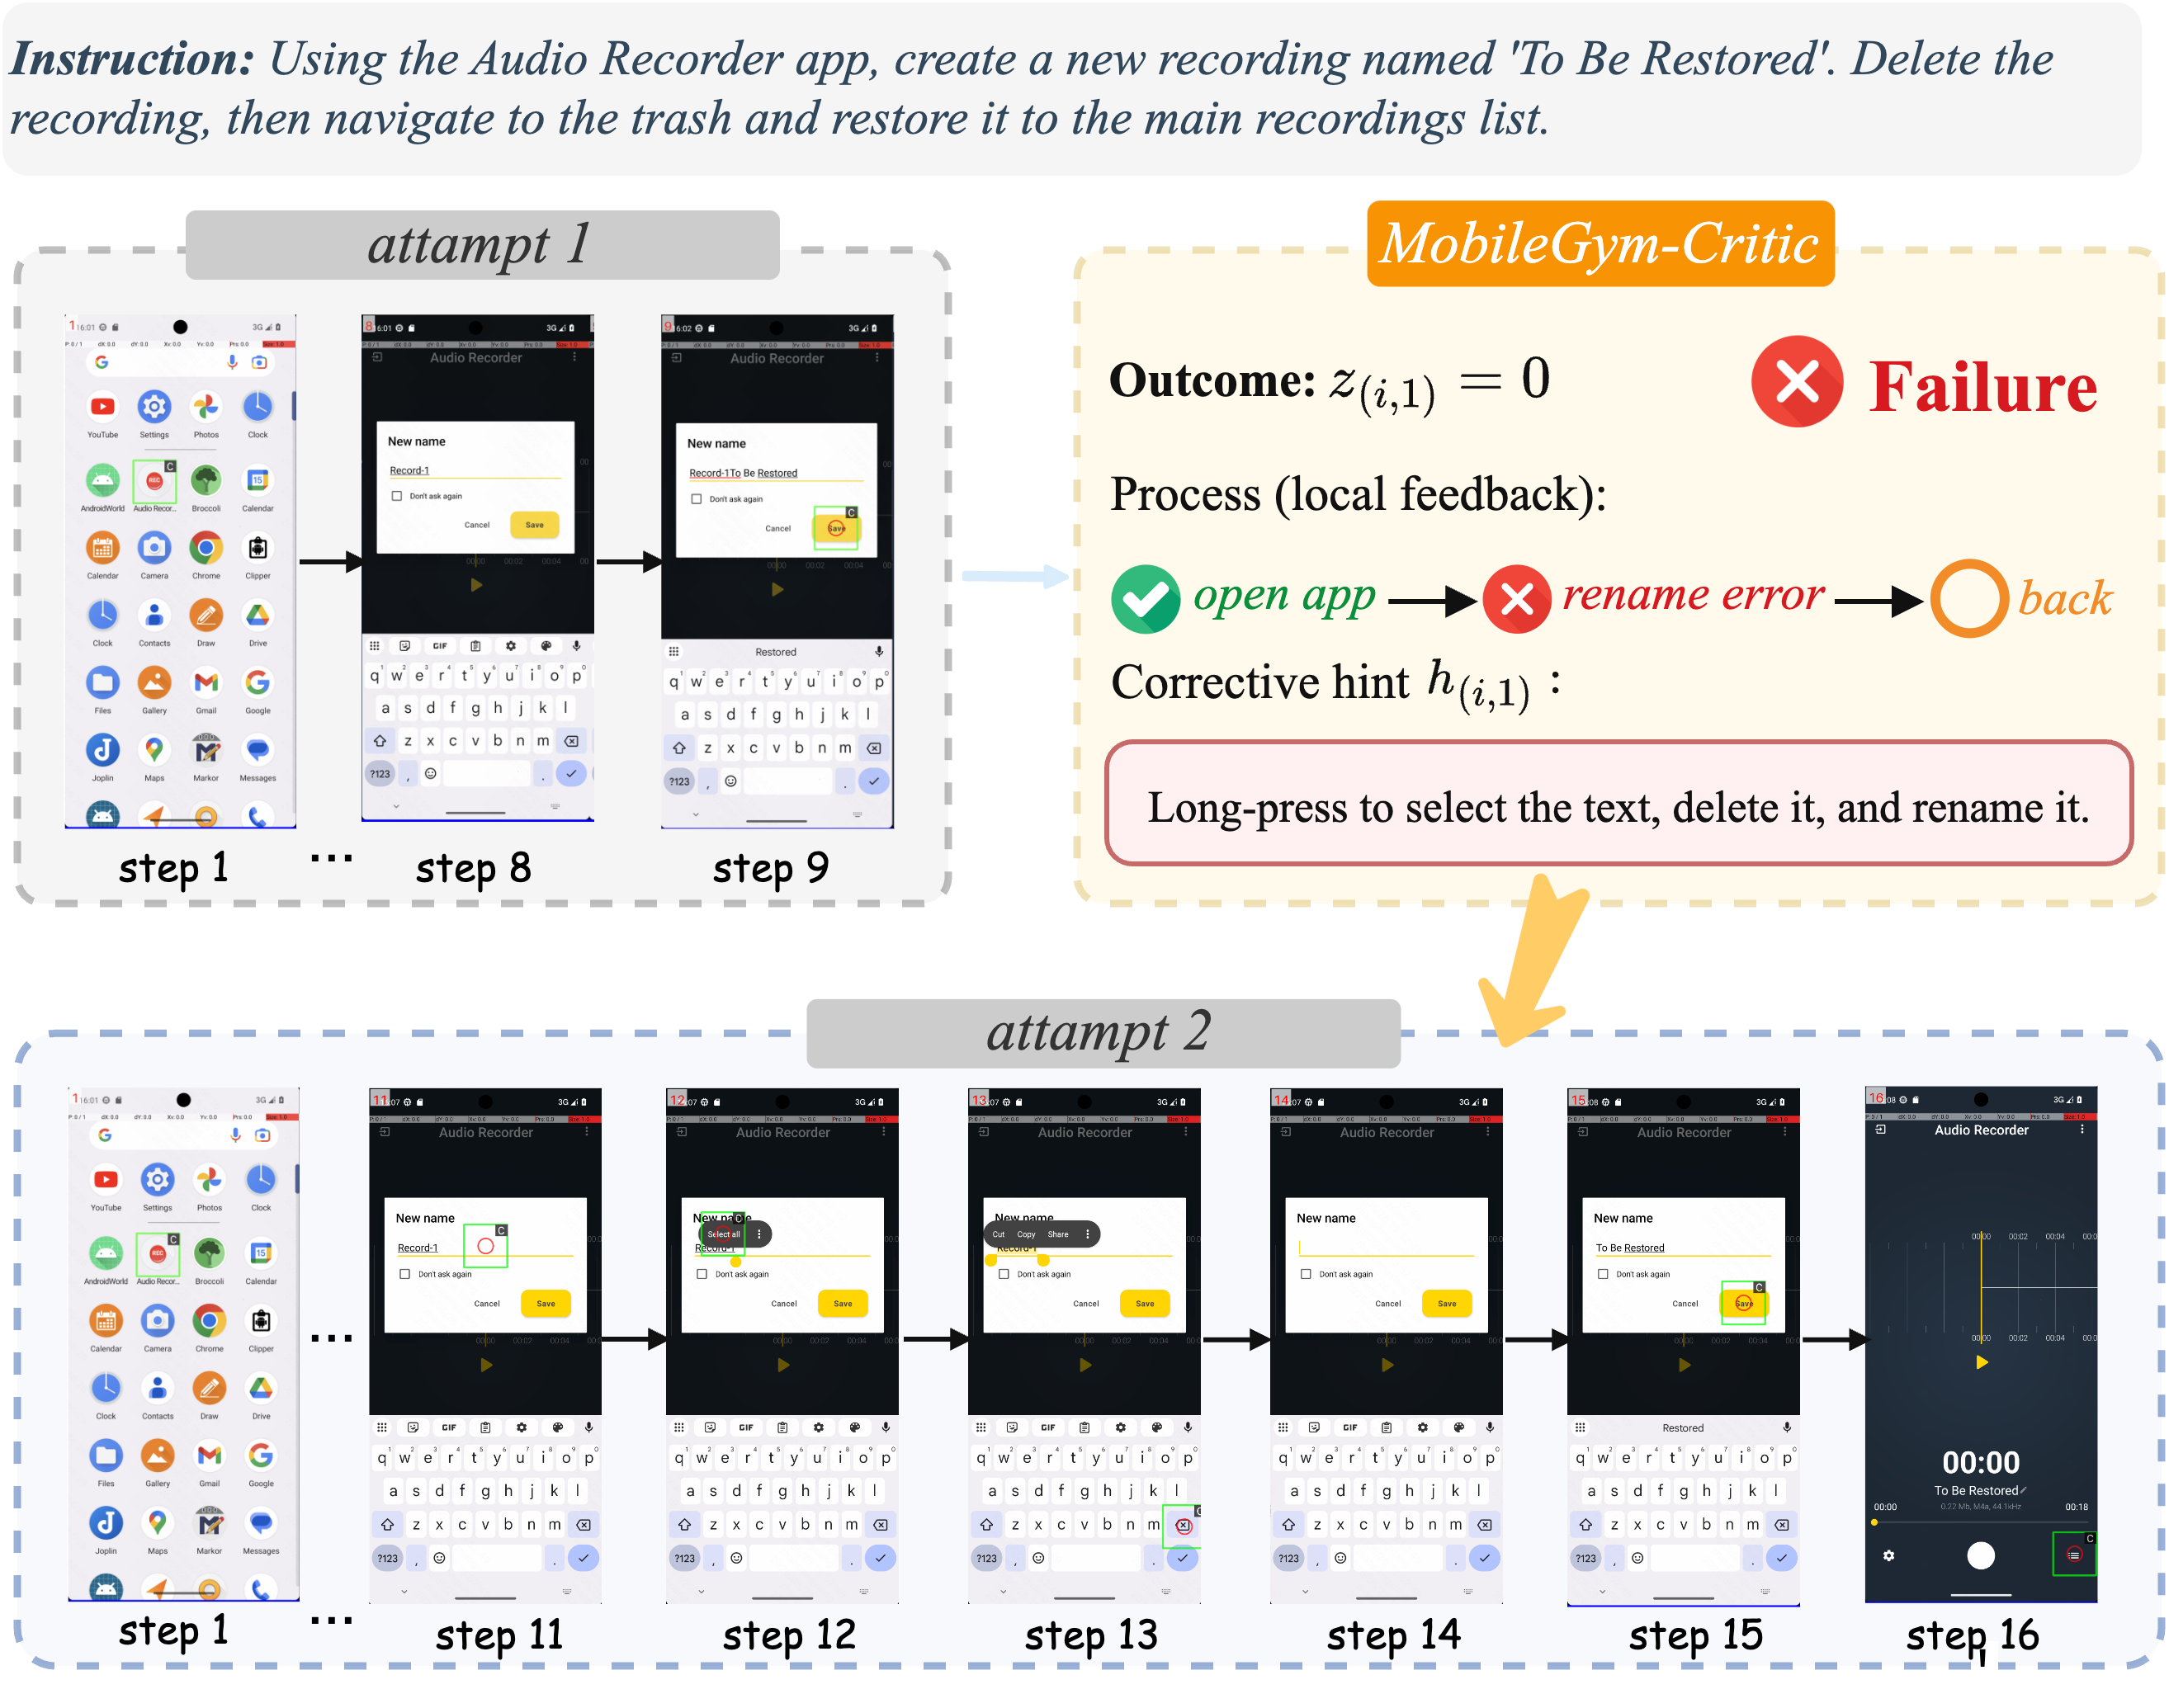
\includegraphics[width=\paperfigmain]{images/case-add-hint/case-study-hint.drawio.png}
    \caption{\textbf{Example of corrective hints improving rollout.}
    A failed or partial attempt can still expose useful app knowledge. \critic summarizes the failure as a compact hint, and later attempts use the hint to avoid repeated mistakes and complete the task more reliably.}
    \label{fig:case-add-hint}
\end{figure}


In implementation, the hint context is appended to the task instruction before the next attempt, while the agent's ordinary screenshot and history fields remain unchanged. For Qwen3-VL, the step prompt follows this protocol:
\begin{lstlisting}[basicstyle=\ttfamily\small,breaklines=true,columns=fullflexible]
The user query: {task instruction}
{evaluation hints from previous attempts}
Task progress: {previous step conclusions}
<image>
\end{lstlisting}
Appendix~\ref{sec:rollout_prompts} gives the core rollout prompt templates for Qwen3-VL and GUI-Owl.

\subsubsection{Task Filtering by Multi-Attempt Success}

For each task, \hifpo computes the empirical success rate across attempts:
\begin{equation}
\label{eq:success-rate}
    \operatorname{SR}(x)=\frac{1}{K}\sum_{k=1}^{K} z_k.
\end{equation}
Tasks with $\operatorname{SR}(x)=1$ are removed because the current policy already solves them consistently. Tasks with $\operatorname{SR}(x)=0$ or $0<\operatorname{SR}(x)<1$ are retained. This choice is deliberate: all-fail tasks can still contain correct local navigation or UI-recognition steps, while partially solved tasks expose unstable decisions that are valuable for adaptation.

\subsubsection{Trajectory and Step Selection}

For every step, we define a reasonable-step indicator from the process label:
\begin{equation}
\label{eq:reasonable-step}
    \chi_k^{(t)}=\mathbb{I}[v_k^{(t)}=1].
\end{equation}
The local quality score of an attempt is the fraction of reasonable steps:
\begin{equation}
\label{eq:quality-score}
    Q_k=\frac{1}{T_k}\sum_{t=1}^{T_k}\chi_k^{(t)}.
\end{equation}
For a retained task, \hifpo selects one informative attempt:
\begin{equation}
\label{eq:attempt-selection}
k^\star(x) =
\begin{cases}
\arg\max_{k:z_k=1} Q_k, & \exists k,\ z_k=1,\\
\arg\max_k Q_k, & \text{otherwise}.
\end{cases}
\end{equation}
Thus, if any attempt succeeds, training uses the successful attempt with the cleanest local process feedback; if all attempts fail, training still uses the failure with the highest fraction of locally reasonable steps.

The step-level training set keeps only reasonable local decisions from the selected attempt:
\begin{equation}
\label{eq:training-set}
    \mathcal{D}=
    \bigcup_{\substack{x\in\mathcal{T}\\ \operatorname{SR}(x)<1}}
    \{(s_{k^\star(x)}^{(t)},a_{k^\star(x)}^{(t)})\mid
    \chi_{k^\star(x)}^{(t)}=1\}.
\end{equation}
Within each set in the union, $s_k^{(t)}$, $a_k^{(t)}$, and $\chi_k^{(t)}$ refer to the rollouts of the current task $x$.
This converts long-horizon mobile trajectories into dense step-level supervision while avoiding the mistake of reinforcing every action in a failed rollout.

\subsubsection{Hint-Contextualized Step-Level GRPO}

After task and step filtering, each training example is a selected local decision rather than a full trajectory. We write it as $d_j=(s_j,a_j^\star)\in\mathcal{D}$, where $a_j^\star=(\alpha_j^\star,\psi_j^\star)$ is the target GUI action selected from a rollout by hierarchical feedback. GRPO was originally introduced as a critic-free policy optimization method that normalizes rewards within a group of responses to the same prompt \citep{shao2024deepseekmath}. Several recent GUI-agent studies adapt this recipe to GUI action prediction by sampling multiple action responses and scoring them with rule-based GUI rewards \citep{lu2025ui,shi2025mobilegui}. \hifpo keeps this group-relative optimization principle, but changes the state on which GRPO operates: the policy is trained on a GUI step augmented with the corrective hint context that was available to the corresponding attempt.

For each sample, the decision state $s_j$ contains the generated task, screenshot observation, interaction history, and corrective hint context $\eta_j$. We render it into a hint-contextualized prompt
\begin{equation}
\label{eq:hint-prompt}
    \tilde{s}_j
    =\operatorname{Prompt}(s_j).
\end{equation}
If no earlier hint exists, $\eta_j=\emptyset$ and $\tilde{s}_j$ reduces to the ordinary step prompt. Otherwise, the prompt exposes compact feedback about what was missed, what should be avoided, or what should be tried next.

The hint is an input condition, not an additional reward term. Thus all responses in the same GRPO group are compared under the same feedback-aware state $\tilde{s}_j$, and the group comparison asks which action is best \emph{given the available correction}. In contrast, a standard step-level GRPO update for GUI action prediction compares actions only under the current screenshot, task, and history. \hifpo therefore makes the group-relative comparison conditional on reusable feedback accumulated across attempts.

For each hint-contextualized step, the old policy samples a group of $G$ candidate responses:
\begin{equation}
\label{eq:hint-grpo-sampling}
    \hat{o}_{j,g}\sim \pi_{\theta_{\rm old}}(\cdot\mid\tilde{s}_j),
    \quad g=1,\ldots,G.
\end{equation}
Each response is parsed into a structured GUI action
$\hat a_{j,g}=\operatorname{Parse}(\hat{o}_{j,g})=(\hat{\alpha}_{j,g},\hat{\psi}_{j,g})$.
Unparseable responses receive zero action reward. For parseable responses, we use an adaptive GUI action reward that separates action type from action arguments:
\begin{equation}
\label{eq:gui-reward}
\begin{aligned}
    r^{\rm type}_{j,g}
    &=\mathbb{I}[\hat{\alpha}_{j,g}=\alpha_j^\star],\\
    r^{\rm arg}_{j,g}
    &=r^{\rm type}_{j,g}\,
      S_{\alpha_j^\star}(\hat{\psi}_{j,g},\psi_j^\star),\\
    R_{j,g}
    &=\lambda_{\rm type}r^{\rm type}_{j,g}
      +\lambda_{\rm arg}r^{\rm arg}_{j,g},
\end{aligned}
\end{equation}
where $\lambda_{\rm type},\lambda_{\rm arg}\geq0$ are reward weights. The type score checks whether the predicted action belongs to the same canonical mobile action as the selected step. The argument score $S_{\alpha_j^\star}\in[0,1]$ is evaluated only when the type is correct, which prevents a wrong action type from receiving credit through accidentally similar parameters. We instantiate $S_{\alpha}$ according to the action semantics: point-in-box or distance-based coordinate matching for click and long-press actions, direction matching for swipes, token-level text similarity for typing or answering, button identity for system actions, status matching for termination actions, and name matching for app-opening or key actions. Wait actions receive full parameter credit after the action type is correct because their training targets do not require an additional argument. Appendix~\ref{sec:appendix_reward} provides the concrete rule-based scoring details. The scalar $R_{j,g}$ is the reward optimized by GRPO; it is distinct from the evaluator labels $z,\ell$ and from the hint context $\eta_j$.

Rewards are normalized within the response group of the same hint-contextualized step. Let
\begin{equation}
\label{eq:group-stats}
\begin{aligned}
    \mu_j&=\frac{1}{G}\sum_{g=1}^{G}R_{j,g},\\
    \sigma_j&=\sqrt{\frac{1}{G}\sum_{g=1}^{G}(R_{j,g}-\mu_j)^2}.
\end{aligned}
\end{equation}
The group-relative advantage is
\begin{equation}
\label{eq:grpo-adv}
    A_{j,g}=
    \frac{R_{j,g}-\mu_j}{\sigma_j+\epsilon_{\rm std}}.
\end{equation}
\hifpo then applies a clipped GRPO update with KL regularization to a reference policy. The response-level importance ratio is
\begin{equation}
\label{eq:grpo-ratio}
\begin{aligned}
    \rho_{j,g}(\theta)=
    \frac{\pi_\theta(\hat{o}_{j,g}\mid\tilde{s}_j)}
         {\pi_{\theta_{\rm old}}(\hat{o}_{j,g}\mid\tilde{s}_j)},\\
    \bar{\rho}_{j,g}(\theta)=
    \operatorname{clip}\!\left(
    \rho_{j,g}(\theta),
    1-\epsilon_{\rm clip},
    1+\epsilon_{\rm clip}
    \right).
\end{aligned}
\end{equation}
The resulting loss is
\begin{equation}
\label{eq:hifpo-objective}
\begin{aligned}
\mathcal{L}_{\hifpo}(\theta)
=&-\mathbb{E}_{j,g}
\left[\min\left(\rho_{j,g}A_{j,g},
\bar{\rho}_{j,g}A_{j,g}\right)\right]\\
&+\beta\,\mathbb{E}_{j}\left[D^{\rm KL}_{j}(\theta)\right].
\end{aligned}
\end{equation}
Here $D^{\rm KL}_{j}(\theta)$ denotes
$D_{\rm KL}\!\left(\pi_\theta(\cdot\mid\tilde{s}_j)\,\|\,\pi_{\rm ref}(\cdot\mid\tilde{s}_j)\right)$, and $\rho_{j,g},\bar{\rho}_{j,g}$ abbreviate the ratios in Equation~\ref{eq:grpo-ratio}.
In short, \hifpo does not replace GRPO with a new optimizer. It makes GRPO step-aware and feedback-aware: trajectory and process feedback choose which local actions become training targets, corrective hints define the conditioning context, and the adaptive GUI reward supplies a verifiable group-relative signal for the sampled actions.

\section{Experiments}
\label{sec:experiments}

\subsection{Experimental Protocol}

\paragraph{Benchmarks.}
We evaluate annotation-free adaptation in two settings. AndroidWorld~\citep{rawles2024androidworld} is the in-domain setting: \ourmethod explores the AndroidWorld app ecosystem, mines adaptation tasks, collects \hifpo rollouts, and evaluates on 116 AndroidWorld tasks with Pass@1, Pass@2, and Pass@3. MobileWorld GUI-only~\citep{kong2026mobileworld} is the out-of-domain setting: we evaluate on its 117-task split and use no MobileWorld rollout, task, or feedback for adaptation.

\paragraph{Base agents and adaptation data.}
We use two 8B-scale instruct base agents: the open generalist \llmname{Qwen3-VL-8B} and the GUI-specialized \llmname{GUI-Owl-1.5-8B}~\citep{bai2025qwen3,xu2026mobile}. \ourmethod generates 3,249 AndroidWorld-side candidate tasks grounded in 527 source trajectory identifiers from 20 apps. To study scaling under realistic compute constraints, we train with 200-, 400-, and 900-task subsets. The main 900-task 8B runs use eight NVIDIA 80GB GPUs and take roughly 80 hours. Appendix~\ref{sec:appendix_data_details} gives the annotation-free adaptation data details, including the generated-task distribution, and Appendix~\ref{sec:appendix_training_details} gives training hyperparameters and reward curves.

\paragraph{Ablation protocol.}
The ablations isolate corrective hints during rollout, hint-contextualized GRPO versus SFT, task-level success-rate filtering, final-decision evaluator choice, and trajectory-grounded curriculum coverage.

\setcounter{insight}{0}

\begin{table*}[!t]
\centering
\paperCompactTable
\begin{paperFit}[\textwidth]
\begin{tabular}{l c c c c c c c c}
\toprule
\multirow{2}{*}{\textbf{Base Agent}} & \multirow{2}{*}{\textbf{Tasks}} & \multicolumn{3}{c}{\textbf{Pass@$k$ Level}} & \multicolumn{3}{c}{\textbf{Task Difficulty Level}} & \multirow{2}{*}{\textbf{Overall Avg.}} \\
\cmidrule(lr){3-5}\cmidrule(lr){6-8}
& & \textbf{Pass@1} & \textbf{Pass@2} & \textbf{Pass@3} & \textbf{Easy} & \textbf{Medium} & \textbf{Hard} & \\
\midrule
\llmname{Qwen3-VL-8B} & 0 & 47/116 (40.5\%) & 57/116 (49.1\%) & 64/116 (55.2\%) & 44.8\% & 35.2\% & \textbf{19.3\%} & 40.7\% \\
\llmname{Qwen3-VL-8B} & 200 & 55/116 (47.4\%) & 64/116 (55.2\%) & 71/116 (61.2\%) & \underline{59.0\%} & 32.4\% & 12.3\% & 44.6\% \\
\llmname{Qwen3-VL-8B} & 400 & \textbf{61/116 (52.6\%)} & \underline{69/116 (59.5\%)} & \underline{73/116 (62.9\%)} & \underline{59.0\%} & \underline{38.9\%} & 14.0\% & \underline{47.8\%} \\
\rowcolor{oursrowcolor}
\llmname{Qwen3-VL-8B} & 900 & \underline{59/116 (50.9\%)} & \textbf{70/116 (60.3\%)} & \textbf{78/116 (67.2\%)} & \textbf{61.2\%} & \textbf{41.7\%} & \underline{17.5\%} & \textbf{49.8\%} \\
\rowcolor{baselinerowcolor}
\multicolumn{2}{r}{\footnotesize\emph{Rel. gain (900 vs. base)}} & \rise{+25.7\%} & \rise{+22.8\%} & \rise{+21.9\%} & \rise{+36.6\%} & \rise{+18.5\%} & \drop{-9.3\%} & \rise{+22.4\%} \\
\midrule
\llmname{GUI-Owl-1.5-8B} & 0 & 65/116 (56.0\%) & 79/116 (68.1\%) & 80/116 (69.0\%) & 66.7\% & 50.0\% & 19.3\% & 54.9\% \\
\llmname{GUI-Owl-1.5-8B} & 200 & \underline{75/116 (64.7\%)} & 85/116 (73.3\%) & \underline{86/116 (74.1\%)} & \underline{73.2\%} & 51.4\% & \underline{28.1\%} & 60.8\% \\
\llmname{GUI-Owl-1.5-8B} & 400 & \underline{75/116 (64.7\%)} & \underline{86/116 (74.1\%)} & \textbf{90/116 (77.6\%)} & \textbf{73.8\%} & \textbf{59.3\%} & 26.3\% & \underline{62.6\%} \\
\rowcolor{oursrowcolor}
\llmname{GUI-Owl-1.5-8B} & 900 & \textbf{78/116 (67.2\%)} & \textbf{87/116 (75.0\%)} & \textbf{90/116 (77.6\%)} & \underline{73.2\%} & \underline{57.4\%} & \textbf{29.8\%} & \textbf{63.4\%} \\
\rowcolor{baselinerowcolor}
\multicolumn{2}{r}{\footnotesize\emph{Rel. gain (900 vs. base)}} & \rise{+20.0\%} & \rise{+10.1\%} & \rise{+12.5\%} & \rise{+9.7\%} & \rise{+14.8\%} & \rise{+54.4\%} & \rise{+15.5\%} \\
\bottomrule
\end{tabular}
\end{paperFit}
\vspace{-1mm}
\caption{AndroidWorld in-domain adaptation and scaling results. Pass@$k$ is computed over 116 tasks. Easy/Medium/Hard report single-attempt success rates by task difficulty. Overall Avg. is the mean of Pass@1/2/3 and Easy/Medium/Hard. Within each base-agent block, best values are bolded and second-best values are underlined. Relative-gain rows compare the 900-task model with the corresponding base agent.}
\label{tab:androidworld_main}
\end{table*}


\subsection{Overall Performance}
\label{sec:results}


\paragraph{In-Domain Adaptation on AndroidWorld.}
Table~\ref{tab:androidworld_main} combines the main AndroidWorld results with the 200/400/900-task scaling study, and Figure~\ref{fig:main-performance}(a) visualizes the same scaling trend. The headline result is that annotation-free adaptation brings the generalist \llmname{Qwen3-VL-8B} close to the closed-data GUI-specialized \llmname{GUI-Owl-1.5-8B}: the adapted model, \llmname{ForgeQwen3-8B}, reaches 67.2\% Pass@3, nearly matching the GUI-Owl base result of 69.0\%. The same loop also improves the stronger GUI-specialized agent. With 900 generated tasks, \llmname{ForgeOwl-8B} reaches 67.2\% Pass@1 and 77.6\% Pass@3. The difficulty columns show where the improvements come from: \ourmethod consistently strengthens easy and medium tasks, and \llmname{ForgeOwl-8B} also improves hard-task single-attempt success from 19.3\% to 29.8\%.



\paragraph{Cross-Domain Generalization to MobileWorld.}
Table~\ref{tab:mobileworld_main} reports out-of-domain MobileWorld GUI-only results. No MobileWorld rollout, task, or feedback is used for adaptation. \llmname{ForgeOwl-8B} reaches 41.0\% success on the 117-task split, surpassing existing open-data mobile GUI agents and approaching much larger or closed-data GUI-specialized systems. \llmname{ForgeQwen3-8B} transfers more modestly, suggesting that out-of-domain generalization still depends strongly on the base agent's mobile GUI competence.

\begin{table}[!htbp]
\centering
\paperTable
\begin{paperFit}
\begin{tabular}{@{}l r@{}}
\toprule
\textbf{Agent} & \textbf{GUI-Only SR (\%)} \\
\midrule
\multicolumn{2}{l}{\textit{\textbf{Open-weight GUI / VLM agents}}} \\
\midrule
\llmname{GUI-Owl-1.5-32B}~\citep{xu2026mobile} & \textbf{43.9} \\
\llmname{MAI-UI-235B-A22B}~\citep{zhou2025mai} & \underline{39.7} \\
\llmname{GUI-Owl-1.5-8B}~\citep{xu2026mobile} & 37.6 \\
\llmname{MAI-UI-32B}~\citep{zhou2025mai} & 36.2 \\
\llmname{GUI-Owl-1.5-2B}~\citep{xu2026mobile} & 32.2 \\
\llmname{MAI-UI-8B}~\citep{zhou2025mai} & 27.5 \\
\llmname{Qwen3-VL-235B-Thinking}~\citep{bai2025qwen3} & 14.5 \\
\llmname{Qwen3-VL-235B}~\citep{bai2025qwen3} & 12.8 \\
\llmname{Qwen3-VL-32B}~\citep{bai2025qwen3} & 11.9 \\
\llmname{Qwen3-VL-8B}~\citep{bai2025qwen3} & 7.6 \\
\midrule
\multicolumn{2}{l}{\textit{\textbf{Open-data mobile GUI agents}}} \\
\midrule
\llmname{OpenMobile-8B}~\citep{OpenMobile2025} & \underline{17.7} \\
\llmname{ClawGUI-2B}~\citep{tang2026clawgui} & 17.1 \\
\llmname{OpenMobile-7B}~\citep{OpenMobile2025} & 14.8 \\
\llmname{ScaleCUA-7B}~\citep{ScaleCUA2025} & 7.7 \\
\rowcolor{oursrowcolor}
\llmname{ForgeQwen3-8B} \textit{(Ours)} & 10.3 \\
\rowcolor{baselinerowcolor}
\multicolumn{1}{r}{\footnotesize\emph{Rel. gain over \llmname{Qwen3-VL-8B}}} & \rise{+35.5\%} \\
\rowcolor{oursrowcolor}
\llmname{ForgeOwl-8B} \textit{(Ours)} & \textbf{41.0} \\
\rowcolor{baselinerowcolor}
\multicolumn{1}{r}{\footnotesize\emph{Rel. gain over \llmname{GUI-Owl-1.5-8B}}} & \rise{+9.0\%} \\
\bottomrule
\end{tabular}
\end{paperFit}
\caption{Out-of-domain MobileWorld GUI-only success rate on the 117-task split. External baseline numbers follow the GUI-only reporting protocol; \ourmethod rows use AndroidWorld-derived adaptation data only. Within each method group, best values are bolded and second-best values are underlined. Relative-gain rows compare each adapted model with its corresponding 8B base agent.}
\label{tab:mobileworld_main}
\end{table}


\insight{\ourmethod improves both generalist and GUI-specialized agents. Its strongest checkpoint, \llmname{ForgeOwl-8B}, achieves the strongest open-data mobile GUI agent result in our evaluation while using only AndroidWorld-side annotation-free adaptation data.}

\subsection{Ablation Analysis}

\begin{table}[!htbp]
\centering
\paperTable
\begin{tabular}{@{}l c c r@{}}
\toprule
\textbf{Metric} & \textbf{No Hint Context} & \textbf{With Corrective Hints} & \textbf{Gain} \\
\midrule
Overall success & 52.0\% & \textbf{77.0\%} & \rise{+25.0 pp} \\
Pass@1 & 30.5\% & \textbf{44.5\%} & \rise{+14.0 pp} \\
Pass@2 & 42.5\% & \textbf{64.0\%} & \rise{+21.5 pp} \\
Pass@3 & 49.0\% & \textbf{72.5\%} & \rise{+23.5 pp} \\
Pass@4 & 52.0\% & \textbf{77.0\%} & \rise{+25.0 pp} \\
Avg. steps / attempt & 18.4 & \textbf{17.2} & \rise{-1.2} \\
Total steps (success only) & 2,593 & \textbf{4,711} & \rise{+2,118} \\
\bottomrule
\end{tabular}
\caption{Trajectory-level rollout ablation on 200 generated tasks with \llmname{Qwen3-VL-8B}. Corrective hints are generated from previous attempts of the same task.}
\label{tab:hint_rollout_ablation_main}
\end{table}


\paragraph{Ablation on corrective rollout hints.}
We remove the corrective hint context from repeated rollout while keeping the same 200 generated tasks. As shown in Table~\ref{tab:hint_rollout_ablation_main}, corrective hints improve overall rollout success from 52.0\% to 77.0\%, Pass@3 from 49.0\% to 72.5\%, and reduce the average steps per attempt. The ablation confirms that multi-attempt rollout becomes useful because feedback accumulates across attempts, not merely because the policy samples more attempts.
\insight{Corrective hints are the bridge between repeated exploration and reusable experience.}

\begin{table}[!htbp]
\centering
\paperTable
\begin{tabular}{@{}l c r@{}}
\toprule
\textbf{Method} & \textbf{Tasks} & \textbf{AndroidWorld Pass@1} \\
\midrule
Base & 0 & 47/116 (40.5\%) \\
No-hint SFT & 200 & 40/116 (34.5\%) \\
Hint SFT & 200 & 53/116 (45.7\%) \\
Hint-contextualized GRPO & 200 & \underline{55/116 (47.4\%)} \\
No-hint SFT & 900 & 51/116 (44.0\%) \\
Hint SFT & 900 & \underline{55/116 (47.4\%)} \\
\rowcolor{oursrowcolor}
Hint-contextualized GRPO & 900 & \textbf{59/116 (50.9\%)} \\
\bottomrule
\end{tabular}
\caption{Training objective ablation with \llmname{Qwen3-VL-8B}. AndroidWorld numbers report Pass@1 over 116 tasks. The best result is bolded and second-best results are underlined.}
\label{tab:training_objective_ablation_main}
\end{table}


\paragraph{Ablation on the training objective.}
We compare SFT and hint-contextualized GRPO on the same generated data, with and without corrective hints. Table~\ref{tab:training_objective_ablation_main} shows that no-hint SFT is weak and can fall below the base model. Hint SFT is better, but hint-contextualized GRPO is strongest at both 200 and 900 tasks, reaching 50.9\% Pass@1 in the 900-task setting. This isolates the value of step-level group-relative optimization after the feedback-guided filtering stage.
\insight{Hint-contextualized GRPO is more effective than direct SFT on the same annotation-free adaptation data.}

\begin{table}[!htbp]
\centering
\paperTable
\begin{tabular}{@{}l c r r r r@{}}
\toprule
\textbf{Filter} & \textbf{SR Range} & \textbf{Samples} & \textbf{Tasks} & \textbf{AW} & \textbf{MW-GUI} \\
\midrule
Medium only & $[0.1,0.9]$ & 1193 & 105 & \textbf{48.3\%} & \underline{12/117} \\
Medium + simple & $[0.1,1.0]$ & 1288 & 120 & \underline{46.6\%} & \textbf{15/117} \\
\rowcolor{oursrowcolor}
Medium + hard & $[0.0,0.9]$ & 1910 & 167 & \textbf{48.3\%} & \textbf{15/117} \\
All tasks & $[0.0,1.0]$ & 2137 & 200 & \textbf{48.3\%} & 10/117 \\
\bottomrule
\end{tabular}
\caption{Task-level success-rate filtering ablation. The final \ourmethod design removes mastered all-success tasks and retains all-fail plus mixed tasks. Best values in result columns are bolded and second-best values are underlined.}
\label{tab:task_filter_ablation_main}
\end{table}


\paragraph{Ablation on task filtering.}
We vary the task-level success-rate range used before step extraction. Table~\ref{tab:task_filter_ablation_main} shows that keeping all-fail and mixed tasks, corresponding to the $[0.0,0.9]$ range, gives the strongest combined AndroidWorld and MobileWorld result among the tested filters. Keeping all tasks admits mastered all-success tasks, while removing all-fail tasks discards useful local progress from difficult attempts.
\insight{The right filtering rule is not to remove failures; it is to remove mastered tasks and let step feedback recover useful local actions.}

\begin{table}[!htbp]
\centering
\paperTable
\begin{tabular}{@{}l c c c r@{}}
\toprule
\textbf{Decision Model} & \textbf{Pass@1} & \textbf{Pass@2} & \textbf{Pass@3} & \textbf{MW-GUI} \\
\midrule
Base, no training & 47/116 & 57/116 & 64/116 & 9/117 \\
\rowcolor{oursrowcolor}
Gemini 2.5 Pro & \textbf{55/116} & \underline{64/116} & \textbf{71/116} & \textbf{15/117} \\
Gemini 3.1 Pro Preview & \underline{52/116} & 62/116 & 69/116 & \underline{13/117} \\
Qwen3-VL-8B & \underline{52/116} & \textbf{67/116} & \underline{70/116} & 11/117 \\
\bottomrule
\end{tabular}
\caption{Final-decision model ablation for \llmname{Qwen3-VL-8B} in the 200-task hint-contextualized GRPO setting. The step-description model is kept fixed. Best values are bolded and second-best values are underlined.}
\label{tab:evaluator_model_ablation_main}
\end{table}


\paragraph{Ablation on the evaluator model.}
We replace the final-decision model used by \critic while keeping the step-description model fixed. Table~\ref{tab:evaluator_model_ablation_main} shows that Gemini 2.5 Pro~\citep{comanici2025gemini} gives the strongest 200-task result, but \llmname{Qwen3-VL-8B} as the decision model still improves the base policy from 40.5\% to 44.8\% Pass@1 and from 55.2\% to 60.3\% Pass@3. Thus, the improvement is not tied to a single proprietary evaluator.
\insight{A stronger evaluator helps, but the \ourmethod feedback-to-optimization loop remains beneficial with a weaker open decision model.}

\begin{table}[!htbp]
\centering
\paperCompactTable
\begin{tabular}{@{}l r r r r@{}}
\toprule
\textbf{Functionality} & \multicolumn{2}{c}{\textbf{Landing-Screen Baseline}} & \multicolumn{2}{c}{\textbf{\ourmethod Curriculum}} \\
\cmidrule(lr){2-3}\cmidrule(lr){4-5}
& \textbf{Count} & \textbf{\%} & \textbf{Count} & \textbf{\%} \\
\midrule
Recipe creation & 49 & 16.3 & 14 & 5.0 \\
Recipe editing & 42 & 14.0 & 35 & 12.5 \\
Recipe deletion & 82 & 27.3 & 4 & 1.4 \\
Search and filter & 25 & 8.3 & 38 & 13.6 \\
Information retrieval / QA & 32 & 10.7 & 20 & 7.1 \\
Favorites & 0 & 0.0 & 3 & 1.1 \\
Shopping list & 0 & 0.0 & 33 & 11.8 \\
Cooking assistant & 0 & 0.0 & 26 & 9.3 \\
Meal planner & 0 & 0.0 & 13 & 4.6 \\
Settings and configuration & 0 & 0.0 & 9 & 3.2 \\
Media and sharing & 0 & 0.0 & 8 & 2.9 \\
Other & 70 & 23.3 & 77 & 27.5 \\
\midrule
Total & 300 & 100.0 & 280 & 100.0 \\
\bottomrule
\end{tabular}
\caption{Functional coverage of Broccoli tasks. Percentages are relative to each generated curriculum.}
\label{tab:curriculum_functional_coverage_main}
\end{table}


\paragraph{Ablation on curriculum grounding.}
Table~\ref{tab:curriculum_functional_coverage_main} compares the functional coverage of tasks generated from only the landing screen against trajectory-grounded \curriculum. The landing-screen baseline over-concentrates on recipe creation, editing, and deletion, with recipe deletion alone taking 27.3\% of tasks. In contrast, \curriculum covers broader functions such as shopping lists, cooking assistant flows, meal planning, settings, and media sharing.
\insight{Exploration grounding matters because it broadens the curriculum beyond functions visible on the first screen.}

\subsection{Case Study and Error Analysis}
\label{sec:case_study_error_analysis}

\begin{figure}[!htbp]
    \centering
    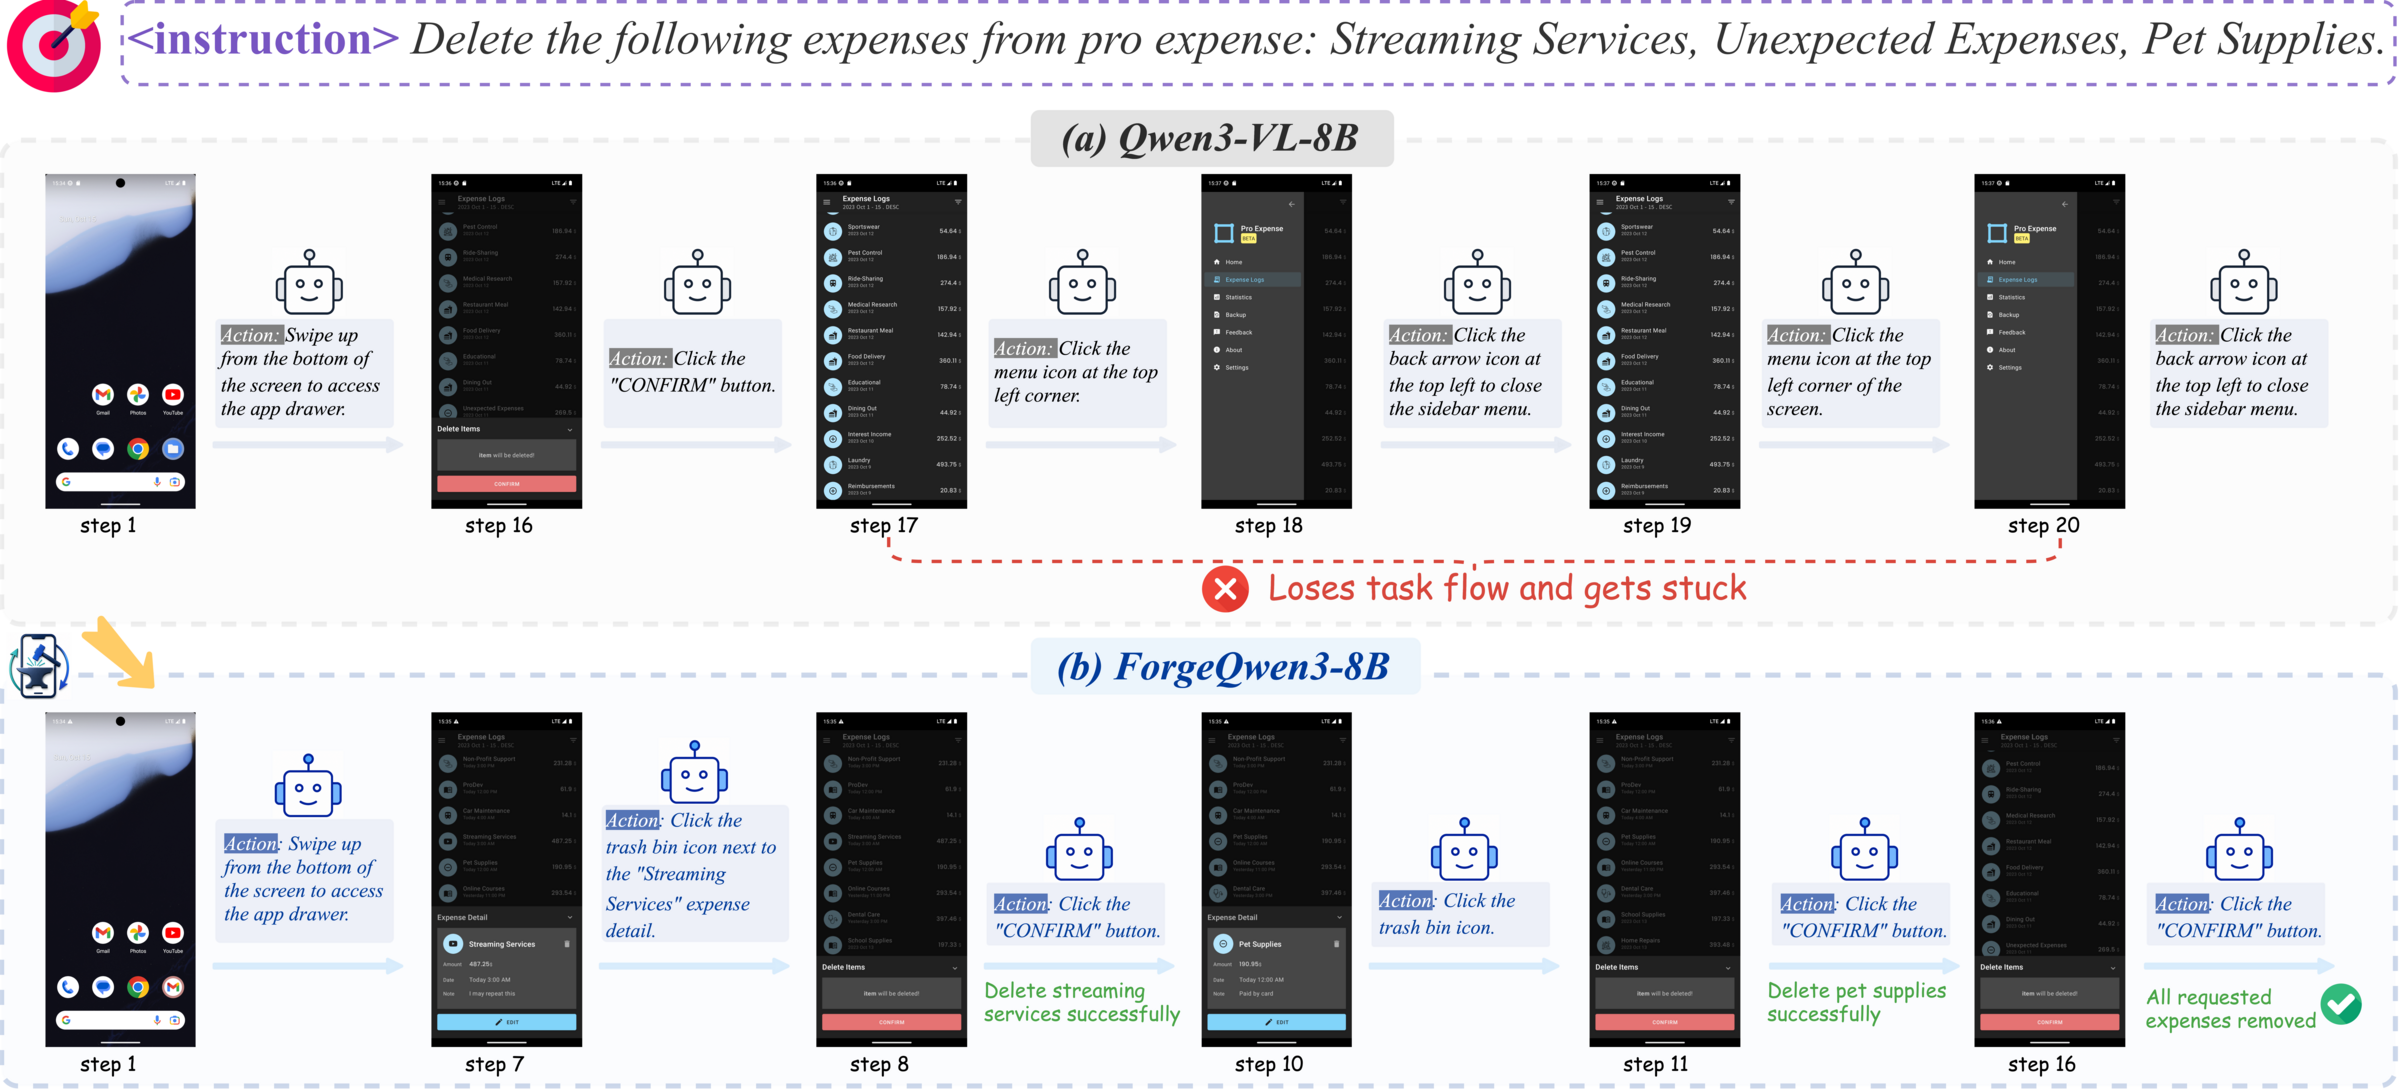
\includegraphics[width=\paperfigmain]{images/case-study/case-study-good-latex.png}
    \caption{\textbf{Case study on AndroidWorld \texttt{ExpenseDeleteMultiple2}.}
    The task asks the agent to delete three expenses from Pro Expense: Streaming Services, Unexpected Expenses, and Pet Supplies. The base \llmname{Qwen3-VL-8B} loses the task flow after an early deletion and gets stuck around the menu/sidebar. The adapted \llmname{ForgeQwen3-8B} follows the task-specific deletion workflow and removes all requested expenses.}
    \label{fig:case-study-good}
\end{figure}


\paragraph{Case Study.}
Figure~\ref{fig:case-study-good} compares \llmname{Qwen3-VL-8B} and the adapted \llmname{ForgeQwen3-8B} on AndroidWorld \texttt{ExpenseDeleteMultiple2}. The base model reaches a deletion confirmation but then loses the task flow, repeatedly opening and closing the sidebar instead of continuing through the remaining requested expenses. After \ourmethod adaptation, \llmname{ForgeQwen3-8B} follows the app-specific deletion pattern across multiple items and completes the requested removals. Additional paired trajectory comparisons in Appendix~\ref{sec:appendix_track_completion_cases} and Figures~\ref{fig:track_completion_androidworld_qwen}, \ref{fig:track_completion_mobileworld_qwen}, and~\ref{fig:track_completion_mobileworld_guiowl} show the same pattern across AndroidWorld and MobileWorld tasks. This example reflects the quantitative gains in Figure~\ref{fig:main-performance}: adaptation mainly improves the agent's ability to preserve task intent across repeated UI procedures.

\begin{figure}[!htbp]
    \centering
    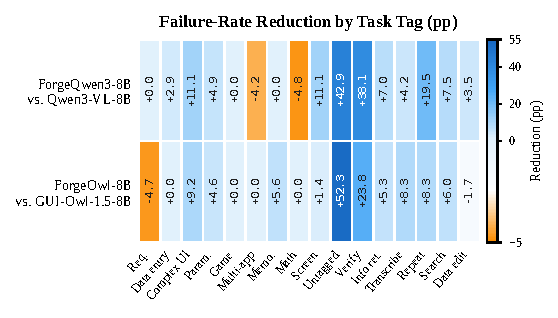
\includegraphics[width=0.7\linewidth]{images/error-analysis-tags/tag-failure-heatmap.pdf}
    \caption{\textbf{AndroidWorld tag-wise failure-rate reduction.}
    Each cell reports the reduction in attempt-level failure rate after \ourmethod adaptation relative to the corresponding base agent; higher is better. Blue cells indicate fewer failures after adaptation, while orange cells indicate regressions.}
    \label{fig:tag_failure_heatmap}
\end{figure}


\paragraph{Error Analysis.}
Figure~\ref{fig:tag_failure_heatmap} visualizes tag-wise failure-rate reduction relative to each base agent. Positive values indicate that \ourmethod reduces failures after adaptation. The largest gains are concentrated in app-grounded UI skills such as verification, search, complex UI understanding, screen reading, repetition, and information retrieval. For example, \llmname{ForgeQwen3-8B} reduces verification failures by 38.1 percentage points, and \llmname{ForgeOwl-8B} reduces search failures by 6.0 percentage points. The remaining hard cases are also clear: game-playing stays unsolved, multi-app tasks do not improve, and memorization/math-counting tasks remain brittle. These failures point to missing long-horizon state, cross-app coordination, and non-standard task-rule coverage rather than simple UI grounding.

\section{Conclusion}

We presented \ourmethod, an annotation-free adaptation system for mobile GUI agents. \ourmethod addresses two bottlenecks in annotation-free GUI learning: the lack of a unified mobile adaptation substrate and the weakness of isolated rollouts with coarse or sparse feedback for long-horizon GUI tasks. \mobilegym grounds task generation and hierarchical rollout evaluation in real target-app interaction, while \hifpo performs multi-attempt hint-guided rollout and transforms evaluated attempts, step-level process feedback, and corrective hints into step-level GRPO updates. Experiments on AndroidWorld and MobileWorld show that \ourmethod improves both an open generalist VLM and a strong GUI-specialized model, with \llmname{ForgeOwl-8B} achieving the strongest open-data mobile GUI agent result in our evaluation. Future work should extend the same feedback-guided adaptation loop to broader app ecosystems, longer multi-app workflows, and more explicit safety constraints for real user devices.

\section{Limitations}

\ourmethod is still bounded by the app ecosystem explored during adaptation. Our main training data comes from AndroidWorld-side apps, so broader app coverage, longer multi-app workflows, persistent user state, and unusual task rules remain challenging. The current system also relies on automatic evaluator quality; stronger or more verifiable critics may further improve safety and reliability on real user devices.


\bibliographystyle{plainnat}
\bibliography{main}


\appendix
\section{Detailed Related Work}
\label{sec:related}

This appendix expands the concise related-work discussion in Section~\ref{sec:introduction}. We organize prior work around the two bottlenecks emphasized in the main paper: the need for a mobile interaction and evaluation substrate, and the need to convert rollout feedback into effective policy optimization signals.

\paragraph{External GUI data construction and trajectory synthesis.}
Several recent systems reduce manual annotation by constructing GUI supervision from external or automatically synthesized sources. TongUI mines multimodal web tutorials and converts them into generalized GUI trajectories across platforms and applications \citep{zhang2025tongui}. MobileA3gent instead uses decentralized user-phone trajectories, automatic intent annotation, and federated training to exploit self-sourced mobile data while preserving user privacy \citep{wang2025mobilea3gent}. OS-Genesis reverses the usual task-first pipeline: it first explores GUI transitions, synthesizes instructions from observed state changes, and filters constructed trajectories with a trajectory reward model \citep{sun2025genesis}. These works substantially reduce the cost of obtaining GUI training data. However, they mainly address data construction. Their supervision is not necessarily grounded in the current state of a target mobile app, and they do not directly connect an agent's own rollout failures to step-level policy improvement.

\paragraph{Autonomous exploration and knowledge mining.}
GUI-explorer is closely related to the exploration side of \ourmethod. It autonomously explores target apps, mines transition-aware knowledge from observation-action-outcome triples, and retrieves that knowledge at inference time to improve GUI grounding and decision making \citep{xie2025gui}. This shows that direct target-app exploration can expose app-specific affordances that static model knowledge misses. The key distinction is the role of the explored knowledge. GUI-explorer is training-free and uses mined knowledge as prompt-side guidance, whereas \ourmethod uses target-app exploration to build an executable curriculum and then continues through rollout execution, hierarchical evaluation, and policy optimization.

\paragraph{Online GUI reinforcement learning.}
ZeroGUI moves GUI learning toward zero-human-cost online RL by automatically generating tasks, estimating trajectory-level success with a VLM evaluator, and updating the GUI policy through online reinforcement learning \citep{yang2025zerogui}. MobileGUI-RL further studies online mobile GUI RL with self-exploration, task filtering, trajectory-aware advantages, and composite rewards that combine success and execution efficiency \citep{shi2025mobilegui}. These works demonstrate that GUI agents can improve through interaction rather than relying only on offline demonstrations. Their optimization signals, however, remain centered on trajectory-level or composite rewards. Such feedback is useful for deciding whether a rollout is good overall, but it provides limited credit assignment for long-horizon mobile tasks where a failed trajectory may still contain useful local decisions and a successful trajectory may include redundant or accidental actions. \ourmethod addresses this by using trajectory outcome feedback, step-level process feedback, and corrective hints for task filtering, trajectory selection, step extraction, and hint-contextualized GRPO.

\paragraph{Self-evolving and continual computer-use agents.}
SEAgent and ACuRL share \ourmethod's motivation that computer-use agents should adapt from their own experience. SEAgent studies self-evolving computer-use agents with a world-state model, curriculum generation, step-wise assessment, guidebook-style experience accumulation, and policy improvement through GRPO and imitation-style objectives \citep{sun2025seagent}. ACuRL formulates environment adaptation as autonomous continual learning: the agent explores an environment, generates curriculum tasks, obtains automatic evaluator feedback, and improves over continual training rounds \citep{xue2026acurl}. These systems are broader computer-use frameworks, primarily designed around desktop or general digital environments. \ourmethod is mobile-specific: \mobilegym provides target mobile app interaction, curriculum mining, rollout execution, and hierarchical mobile rollout evaluation, while \hifpo schedules multi-attempt rollout, reuses corrective hints across attempts, and performs hint-contextualized step-level GRPO.

\paragraph{Synthetic GUI environmental dynamics.}
UI-Oceanus scales GUI agents by synthesizing environmental dynamics and training on transition-oriented objectives \citep{wu2026uioceanus}. This line improves the coverage of GUI state transitions without requiring every transition to be manually collected in the target environment. It is complementary to \ourmethod: synthetic dynamics can broaden pretraining or supervised training data, while \ourmethod focuses on annotation-free adaptation inside target mobile apps, where the agent must discover executable tasks, evaluate its own rollouts, and update from the resulting experience.

\paragraph{Positioning of \ourmethod.}
Taken together, prior work has made GUI learning less dependent on human-written demonstrations, but two bottlenecks remain for mobile target-app adaptation. External data construction provides scalable supervision but may not reflect the current target app. Exploration methods expose app-specific knowledge but often stop at inference-time guidance. Online RL methods update the policy but usually rely on coarse trajectory feedback. Continual computer-use methods study self-evolution but are not designed as mobile-specific interaction and evaluation substrates. \ourmethod addresses these gaps by separating the system into two roles. \mobilegym supplies the mobile substrate: target-app exploration, executable curriculum mining, rollout execution, and hierarchical feedback. \hifpo supplies the feedback-to-optimization mechanism: it schedules multi-attempt rollout, accumulates corrective hints, filters mastered tasks, selects informative trajectories and steps, and optimizes the policy with hint-contextualized step-level GRPO. Table~\ref{tab:related_work_comparison} summarizes this comparison.

\begin{table*}[t]
\centering
\paperCompactTable
\begin{paperFit}[\textwidth]
\begin{tabular}{l l c c c l c l}
\toprule
\textbf{Method} &
\textbf{Main Source / Setting} &
\multicolumn{3}{c}{\textbf{Pain Point 1: Mobile Interaction and Evaluation Substrate}} &
\multicolumn{3}{c}{\textbf{Pain Point 2: Feedback-to-Optimization}} \\
\cmidrule(lr){3-5} \cmidrule(lr){6-8}
&
&
\makecell{\textbf{Target Mobile}\\\textbf{Interaction}} &
\makecell{\textbf{Auto Task /}\\\textbf{Curriculum}} &
\makecell{\textbf{Hierarchical}\\\textbf{Rollout Eval.}} &
\makecell{\textbf{Feedback}\\\textbf{Granularity}} &
\makecell{\textbf{Cross-Attempt}\\\textbf{Experience}} &
\makecell{\textbf{Policy}\\\textbf{Update}} \\
\midrule
TongUI & Web tutorials & \pmark & \xmark & \xmark & Tutorial-derived trajectories & \xmark & SFT \\
MobileA3gent & User phone trajectories & \pmark & \xmark & \xmark & Auto-annotated instructions & \xmark & SFT / FL \\
GUI-explorer & Autonomous app exploration & \cmark & \pmark & \xmark & Transition-aware knowledge & \pmark & \xmark \\
OS-Genesis & Reverse task synthesis & \pmark & \cmark & \pmark & Trajectory reward model & \xmark & SFT \\
ZeroGUI & Online GUI rollout & \pmark & \cmark & \pmark & Trajectory-level VLM reward & \xmark & Online RL \\
MobileGUI-RL & Online mobile rollout & \cmark & \cmark & \pmark & Trajectory-level composite reward & \xmark & MobiGRPO \\
SEAgent & Desktop software & \xmark & \cmark & \pmark & Step-wise assessment & \pmark & GRPO + imitation \\
ACuRL & Computer-use environments & \xmark & \cmark & \pmark & Outcome evaluator / CUAJudge & \pmark & Curriculum RL \\
UI-Oceanus & Synthetic GUI dynamics & \pmark & \cmark & \xmark & Transition objectives & \xmark & CPT + SFT \\
\midrule
\rowcolor{oursrowcolor}
\textbf{\ourmethod} &
\textbf{Target mobile apps} &
\cmark &
\cmark &
\cmark &
\makecell[l]{\textbf{Trajectory outcome}\\\textbf{+ step-level process}\\\textbf{+ corrective hints}} &
\cmark &
\textbf{\hifpo} \\
\bottomrule
\end{tabular}
\end{paperFit}
\vspace{2pt}
\begin{flushleft}
\footnotesize
\cmark: explicitly supported; \pmark: partially supported or not specific to annotation-free mobile adaptation; \xmark: not supported or not the focus. \mobilegym covers the interaction and evaluation substrate, while \hifpo covers cross-attempt experience reuse and policy optimization.
\end{flushleft}
\caption{Comparison with annotation-free GUI agent learning and adaptation methods. We organize the comparison around two limitations addressed by \ourmethod: the lack of a unified mobile interaction and evaluation substrate, and the reliance on isolated rollout experience with coarse or sparse feedback.}
\label{tab:related_work_comparison}
\end{table*}


\section{Method Notation and Algorithm}
\label{sec:appendix_method_details}

Table~\ref{tab:method_notation} lists the main symbols used in Section~\ref{sec:method}. Algorithm~\ref{alg:mobileforge} gives a compact procedural view of the annotation-free adaptation loop.

\begin{table}[t]
\centering
\paperTable
\begin{tabular}{L{0.23\linewidth} L{0.66\linewidth}}
\toprule
\textbf{Symbol} & \textbf{Meaning} \\
\midrule
$\mathcal{E}$ & Target mobile app environment. \\
$\mathcal{Z}$ & Exploration evidence collected from target apps. \\
$\mathcal{T}$ & Generated adaptation curriculum. \\
$x$ & A generated task in curriculum $\mathcal{T}$. \\
$\tau_k$ & The $k$-th rollout attempt for task $x$. \\
$\eta_{<k}$ & Corrective hint context from earlier attempts of task $x$. \\
$\mathcal{F}_{k}$ & Hierarchical feedback for attempt $\tau_k$. \\
$I_k^{(t)}$ & Screenshot observation at attempt $k$ and step $t$. \\
$s_k^{(t)}$ & Decision state at attempt $k$ and step $t$. \\
$a_k^{(t)}=(\alpha,\psi)$ & Structured GUI action with type $\alpha$ and arguments $\psi$. \\
$z_k$ & Trajectory outcome label; $1$ means task success and $0$ means failure. \\
$\ell_k^{(t)}$ & Step-level process label. \\
$v_k^{(t)}$ & Binary reasonableness label for step $t$ in attempt $k$. \\
$e_k^{(t)}$ & Natural-language rationale for the step-level label. \\
$\chi_k^{(t)}$ & Indicator that a step is marked reasonable by \critic. \\
$Q_k$ & Local quality score of attempt $\tau_k$. \\
$h_k$ & Corrective hint generated after an attempt. \\
$d_j=(s_j,a_j^\star)$ & Step-level training sample and selected action. \\
$\tilde{s}_j$ & Hint-contextualized prompt used by step-level GRPO. \\
$R_{j,g}$ & Adaptive GUI action reward for candidate $g$ in a GRPO group. \\
\bottomrule
\end{tabular}
\caption{Key notation used in the method.}
\label{tab:method_notation}
\end{table}


\begin{algorithm}[t]
\caption{\ourmethod annotation-free adaptation loop}
\label{alg:mobileforge}
\KwIn{Target apps $\mathcal{E}$, policy $\pi_\theta$, attempts per task $K$}
\KwOut{Adapted policy $\pi_{\theta'}$}
Explore target apps and record reachable GUI transitions\;
Generate trajectory-grounded tasks from the explored transitions\;
\ForEach{task $x\in\mathcal{T}$}{
    initialize hint context $\eta_{<1}\leftarrow\emptyset$\;
    \For{$k=1$ \KwTo $K$}{
        run attempt $\tau_k$ with policy $\pi_\theta$ and hints $\eta_{<k}$\;
        evaluate the attempt to obtain outcome label $z$, step labels $\ell$, and hint $h$\;
        update the hint context for later attempts\;
    }
}
Remove mastered tasks, select informative attempts, and extract useful local steps\;
Train the policy with hint-contextualized step-level GRPO\;
\Return{$\pi_{\theta'}$}\;
\end{algorithm}

\section{Pipeline Details}
\label{sec:appendix_pipeline}

Table~\ref{tab:appendix_pipeline} summarizes the main system stages and their inputs and outputs.

\begin{table}[t]
\centering
\paperTable
\begin{tabular}{@{}l l l@{}}
\toprule
\textbf{Stage} & \textbf{Input} & \textbf{Output} \\
\midrule
Target exploration & Target apps & Exploration evidence \\
Curriculum generation & Exploration evidence & Executable task curriculum \\
HiFPO hint-guided rollout & Tasks and current policy & Multi-attempt trajectories \\
MobileGym hierarchical evaluation & Completed trajectories & Outcome feedback, process feedback, hints \\
Step-level filtering & Tasks, trajectories, feedback & Filtered step-level training samples \\
Policy optimization & Step-level samples & Adapted policy \\
\bottomrule
\end{tabular}
\caption{Pipeline stages used by \ourmethod.}
\label{tab:appendix_pipeline}
\end{table}

\paragraph{Filtering order.}
The task-level success-rate filter is applied before best-trajectory selection. This matters because the task success rate must be computed from the original multi-attempt task group. The main setting uses $\operatorname{SR}_{\min}=0.0$ and $\operatorname{SR}_{\max}<1.0$, which removes all-success mastered tasks and keeps all-fail and partially solved tasks. Best-trajectory selection and reasonable-step filtering are then applied to extract useful local decisions.

\section{Experimental Protocol Details}
\label{sec:appendix_experimental_protocol}

\paragraph{Benchmarks.}
AndroidWorld~\citep{rawles2024androidworld} is the in-domain setting: \ourmethod explores the AndroidWorld app ecosystem, mines adaptation tasks, collects \hifpo rollouts, and evaluates on 116 AndroidWorld tasks with Pass@1, Pass@2, and Pass@3. MobileWorld GUI-only~\citep{kong2026mobileworld} is the out-of-domain setting: we evaluate on its 117-task split and use no MobileWorld rollout, task, or feedback for adaptation.

\paragraph{Base agents and adaptation scale.}
We use two 8B-scale instruct base agents: the open generalist \llmname{Qwen3-VL-8B} and the GUI-specialized \llmname{GUI-Owl-1.5-8B}~\citep{bai2025qwen3,xu2026mobile}. \ourmethod generates 3,249 AndroidWorld-side candidate tasks grounded in 527 source trajectory identifiers from 20 apps. To study scaling under realistic compute constraints, we train with 200-, 400-, and 900-task subsets. The main 900-task 8B runs use eight 80GB GPUs and take roughly 80 hours.

\paragraph{Ablation scope.}
The ablations isolate corrective hints during rollout, hint-contextualized GRPO versus SFT, task-level success-rate filtering, final-decision evaluator choice, and trajectory-grounded curriculum coverage.

\section{Annotation-Free Adaptation Data Details}
\label{sec:appendix_data_details}

Table~\ref{tab:generated_task_corpus} reports the generated AndroidWorld-side adaptation task pool by source app. The full pool contains 3,249 candidate tasks grounded in 527 source trajectory identifiers from 20 apps.

\begin{table}[!htbp]
\centering
\paperTable
\begin{tabular}{@{}l r@{\qquad\qquad}l r@{}}
\toprule
\textbf{App} & \textbf{\#Tasks} & \textbf{App} & \textbf{\#Tasks} \\
\midrule
Files & 258 & Tasks & 150 \\
Pro Expense & 247 & Simple Draw Pro & 145 \\
Broccoli Recipe & 241 & OsmAnd & 136 \\
Simple SMS Messenger & 240 & Joplin & 130 \\
Markor & 233 & Simple Calendar Pro & 107 \\
Clock & 215 & OpenTracks & 104 \\
Retro Music & 189 & Settings & 102 \\
Contacts & 166 & Camera & 94 \\
VLC & 161 & Audio Recorder & 91 \\
Chrome & 157 & Simple Gallery Pro & 83 \\
\bottomrule
\end{tabular}
\caption{Generated AndroidWorld-side adaptation tasks by source app. The full pool contains 3,249 candidate tasks grounded in 527 source trajectory identifiers from 20 apps.}
\label{tab:generated_task_corpus}
\end{table}


\section{Exploration Phase Details}
\label{sec:exploration_details}

\mobilegym begins by collecting raw interaction evidence from each target app. We adopt a function-aware exploration strategy inspired by GUI-explorer~\citep{xie2025gui}, replacing unguided random walks with app-grounded goal generation and systematic traversal.

\paragraph{Exploration anchors.}
For an Android app, the explorer extracts structural anchors from app metadata, especially the activity list declared by the APK. These anchors provide a compact description of reachable app functions and screens. They do not serve as demonstrations; they only ground exploration goals in functions that the app plausibly exposes.

\paragraph{Function-aware goal generation.}
At each exploration state, an MLLM receives the current screenshot together with the app name, package name, and available activity anchors. It generates concrete user goals that start from the current screen, are expected to be executable within a bounded number of steps, and cover diverse interaction patterns such as viewing, editing, searching, sharing, configuration, and information lookup. This design makes the explored trajectories more likely to touch real app functions than generic task templates.

\paragraph{Depth-first trajectory collection.}
The explorer pursues generated goals with depth-first traversal. When branching to a new goal from an earlier state, it restores the parent state by relaunching the app and replaying the parent action prefix, then continues exploration from that state. For each transition, it records the task goal, before/after screenshots, selected action, target element, execution metadata, and a short summary. The output is a rich but unstructured evidence pool $\mathcal{Z}$ used by \curriculum to mine executable adaptation tasks.

\section{Prompt Templates}
\label{sec:appendix_prompts}

\subsection{Curriculum Generation Prompt}
\label{sec:curriculum_prompt}

The \curriculum prompt jointly performs trajectory assessment and task generation. The model observes the original exploration goal, visualized screenshots from the trajectory, few-shot task examples, task-generation principles, and already generated tasks for the same app. The core template is shown below.

\begin{promptlistingbox}[MobileGym-Curriculum core prompt]
You are an expert Curriculum Generator - a teacher designing
comprehensive learning tasks for GUI agents. Your core purpose is to
create a complete curriculum covering all app functionalities with
progressive difficulty levels to systematically teach GUI agents how
to use the target app.

Your job is to:
1. EVALUATE the original task for reasonableness and completion.
2. GENERATE new diverse curriculum tasks that comprehensively cover
   the app's functionality.

## App Information
App Name: {app_name}
Original Task Goal: {original_goal}

## Few-shot Examples
{fewshot_examples}

## Task Generation Principles
{task_principles}

## Already Generated Tasks for {app_name}
{existing_tasks}
IMPORTANT: Do not generate tasks that are too similar to the above.

## Curriculum Design Instructions

### Step 1: Task Evaluation
1. Reasonableness Assessment:
   - Is this a reasonable task that a user might actually want to
     perform in this app?
   - Are the requirements clear and achievable?
   - Does the task make sense in the context of the app?

2. Step-by-Step Quality Analysis:
   - Analyze representative visible steps in the screenshot sequence.
   - A reasonable step logically progresses toward task completion.
   - An unreasonable step is unnecessary, wrong, counterproductive,
     stuck in a loop, or moves backward unnecessarily.
   - Failed trajectories may contain reasonable steps.
   - Successful trajectories may contain detours or inefficiencies.
   - Compute trajectory_quality_score = reasonable_steps / total_steps.

3. Overall Completion Assessment:
   - Did the agent complete the stated task?
   - Were the required steps performed correctly?
   - Did the agent reach the intended goal state?

### Step 2: Curriculum Task Generation
Generate 3-8 new learning tasks that:
- cover different core functionalities of {app_name};
- vary in length from 1 to 40 steps;
- are pedagogically useful for teaching GUI agents;
- avoid redundancy with existing tasks;
- focus on core functionality variations, not only parameter changes;
- limit each functionality to at most 3 parameter variations.

## Output Format
Return JSON:
{
  "evaluation": {
    "task_reasonable": true/false,
    "task_completed": true/false,
    "reasonableness_explanation": "...",
    "completion_explanation": "...",
    "confidence_score": 0.0-1.0,
    "step_quality_analysis": {
      "total_steps": 10,
      "reasonable_steps": 8,
      "trajectory_quality_score": 0.8,
      "quality_summary": "..."
    }
  },
  "generated_tasks": [
    {
      "task_id": "task_1",
      "instruction": "Self-contained learning task",
      "estimated_steps": 5,
      "core_functionality": "Main functionality being taught",
      "variation_type": "simplification/parameter_change/"
                        "scenario_application/step_progression",
      "prerequisites": "Only non-obvious prerequisites"
    }
  ]
}
\end{promptlistingbox}

\subsection{MobileGym-Critic Prompts}
\label{sec:critic_prompts}

\critic uses a hierarchical prompting procedure. The first prompt converts each visualized action into a compact step description. The second prompt makes the final trajectory decision and step-level process assessment. The third prompt turns failures or inefficient steps into corrective hints for later attempts.

\begin{promptlistingbox}[MobileGym-Critic step description prompt]
System:
You are an expert mobile device assistant. Analyze a two-panel image
showing the Before Action and After Action state of a user's workflow.
Focus only on the Before Action panel. Output JSON.

User:
The overall task is: {task_description}

The image shows a before/after action state. The user action is
visualized with markers, and the raw action log is:
- Action Type: {log_action}
- Action Detail: {log_detail}

Return JSON:
{
  "action_description": "A crisp description of the action performed",
  "ui_description": "Task-relevant UI elements visible before the action"
}
\end{promptlistingbox}

\begin{promptlistingbox}[MobileGym-Critic final decision prompt]
System:
You are an expert in evaluating mobile UI automation tasks.
Use the evaluation guidelines:
- The final UI state must satisfy all task requirements.
- Existing conditions can satisfy requirements without repetition.
- A logically correct action sequence can imply success even if the
  last screen alone is insufficient.
- The agent may make and correct mistakes.
- If a task is inherently infeasible, the agent can still succeed by
  correctly identifying the impossibility and giving appropriate feedback.

User:
Task Description: {task_description}

Here is a step-by-step breakdown of the agent's actions, including raw
action logs and VLM-generated descriptions:
{step_descriptions_with_raw_logs}

You are also provided with a composite image of the last screenshots.
Synthesize the visual evidence with the full step list.

Required assessment:
1. Decide whether the attempt completed the task.
2. Assess whether the task itself is feasible.
3. If failed, identify the failure_step.
4. Analyze every step for reasonableness and provide a concise rationale.

Return JSON:
{
  "decision": 1 or 0,
  "reason": "Explanation of the final judgment",
  "failure_step": 4,
  "task_feasible": true/false,
  "task_feasible_reason": "Why the task is feasible or infeasible",
  "task_barriers": [],
  "reasonable_steps": [1, 2, 4],
  "unreasonable_steps": [3],
  "step_analysis": {
    "1": {
      "reasonableness": "reasonable",
      "explanation": "..."
    },
    "3": {
      "reasonableness": "unreasonable",
      "explanation": "..."
    }
  }
}
\end{promptlistingbox}

\begin{promptlistingbox}[MobileGym-Critic corrective hint prompt]
System:
You are an intelligent agent performing self-reflection on your task
execution. Analyze your own actions, identify mistakes and
inefficiencies, and extract lessons for future attempts. Use the
step-by-step reasonableness analysis. Output JSON.

User:
## Task
{task_description}

## My Steps (with Reasonableness Analysis)
{step_descriptions_with_step_analysis}

## Evaluation Result
{failure_or_inefficiency_reason}

Reflect on the execution:
1. Identify key mistakes, especially unreasonable steps.
2. Specify what to avoid in future attempts.
3. Propose concrete alternative approaches.
4. Extract important task insights.

Return JSON:
{
  "key_mistake": "Concise summary of the main mistake",
  "what_to_avoid": ["..."],
  "suggested_approach": ["..."],
  "important_insights": ["..."],
  "hint_summary": "Brief self-reminder for the next attempt"
}
\end{promptlistingbox}

\subsection{Hint-Guided Rollout Prompts}
\label{sec:rollout_prompts}

During \hifpo rollout, the hint context $\eta_{<k}$ is appended to the task instruction before attempt $k$. The same mechanism is used for both base agents; the difference lies in each agent's native step prompt. The shared hint block has the following structure.

\begin{promptlistingbox}[Corrective hint context block]
EVALUATION HINTS FROM PREVIOUS ATTEMPTS
The following insights come from analysis of previous failed attempts.
Please review these carefully to avoid repeating the same mistakes:

--- Hint from Attempt #{attempt_id} ---
Summary: {hint_summary}
Key Mistake: {key_mistake}
What to Avoid:
  - {avoid_item_1}
  - {avoid_item_2}
Suggested Approach:
  - {approach_item_1}
  - {approach_item_2}
Important Insights:
  - {insight_item_1}

END OF EVALUATION HINTS
\end{promptlistingbox}

For Qwen3-VL, the structured hint block is inserted into the query field, while the screenshot remains the visual observation for the current step.

\begin{promptlistingbox}[Qwen3-VL hint-contextualized rollout prompt]
System:
You are a helpful assistant that can help with tasks on a mobile device.
Use the mobile_use tool with actions such as click, long_press, swipe,
type, answer, system_button, wait, and terminate.
Return exactly:
  <thinking>...</thinking>
  <tool_call>{"name": "mobile_use", "arguments": {...}}</tool_call>
  <conclusion>UI observation: ... Intended action: ...</conclusion>
If the task is completed, terminate with status="success"; if it is
infeasible, terminate with status="failure". Trust the current UI state
over action history. If hints are present in the task description, use
them to avoid repeating previous mistakes.

User:
The user query: {task_instruction}
{EVALUATION_HINTS_FROM_PREVIOUS_ATTEMPTS}

Task progress (You have done the following operation on the current
device):
{previous_step_conclusions}
<image>
\end{promptlistingbox}

For GUI-Owl, the hint block is likewise appended to the instruction, while the prompt preserves GUI-Owl's concise action-plus-tool-call format.

\begin{promptlistingbox}[GUI-Owl hint-contextualized rollout prompt]
System:
You may use the mobile_use tool with actions such as key, click,
long_press, swipe, type, system_button, open, wait, answer, and
terminate. For each step, output:
  Action: {short imperative}
  <tool_call>{"name": "mobile_use", "arguments": {...}}</tool_call>

User:
Please generate the next move according to the UI screenshot,
instruction and previous actions.

Instruction: {task_instruction}
{EVALUATION_HINTS_FROM_PREVIOUS_ATTEMPTS}

Previous actions:
{action_history_or_no_previous_action}
<image>
\end{promptlistingbox}

\section{Adaptive GUI Action Reward}
\label{sec:appendix_reward}

The step-level GRPO stage uses a rule-based GUI action reward. For each hint-contextualized prompt, the policy samples a group of responses. Each response is first parsed into a structured action $\hat a=(\hat\alpha,\hat\psi)$ and compared against the selected action $a^\star=(\alpha^\star,\psi^\star)$ extracted from hierarchical feedback. The parser supports the output templates used by both base agents and maps action aliases into a canonical mobile action space before scoring.

The optimized scalar reward is
\begin{equation}
\label{eq:appendix_reward}
R(\hat a,a^\star)
=\lambda_{\rm type}r_{\rm type}
+\lambda_{\rm arg}r_{\rm arg},
\end{equation}
where $\lambda_{\rm type}$ and $\lambda_{\rm arg}$ are configurable weights. The implementation also logs a binary format score for malformed tool calls, but this format score is not included in $R$. The type score is
\begin{equation}
\label{eq:appendix_type_reward}
r_{\rm type}=\mathbb{I}[\hat\alpha=\alpha^\star].
\end{equation}
The argument score is gated by the type score:
\begin{equation}
\label{eq:appendix_arg_reward}
r_{\rm arg}=
\begin{cases}
S_{\alpha^\star}(\hat\psi,\psi^\star), & r_{\rm type}=1,\\
0, & r_{\rm type}=0.
\end{cases}
\end{equation}
Thus a response with the wrong action type receives no parameter credit. The main experiments use the reward weights reported in Section~\ref{sec:experiments}; the same reward implementation exposes these weights as hyperparameters.

\begin{table}[t]
\centering
\paperTable
\begin{tabular}{p{0.20\linewidth} p{0.70\linewidth}}
\toprule
\textbf{Action} & \textbf{Argument score} \\
\midrule
click & If the target is a box, reward is $1$ when the predicted point is inside the box; otherwise it decays with distance to the box center normalized by the box diagonal. If the target is a point, reward is $\max(0,1-d/50)$ in the normalized 0--1000 coordinate space. \\
long press & Same coordinate score as click. \\
swipe & If a target direction is provided, reward is $1$ only when the predicted direction matches. If no target direction is provided, a valid swipe parameter receives full credit. \\
type & Token-level F1 similarity between predicted text and target text. \\
answer & Token-level F1 similarity when a target answer is provided; otherwise full credit after the action type is correct. \\
system button & Exact match of the system button identity, such as Back, Home, Menu, or Enter. \\
wait & Full credit after the action type is correct; no additional argument is required by the training target. \\
terminate & Exact match of the termination status when one is provided; otherwise full credit after the action type is correct. \\
open & Exact app-name match receives full credit; containment-based partial app-name match receives partial credit. If no target app name is provided, the argument score is treated as satisfied. \\
key & Exact key-name match when one is provided; otherwise full credit after the action type is correct. \\
\bottomrule
\end{tabular}
\caption{Rule-based argument score $S_{\alpha}$ used by the adaptive GUI action reward.}
\label{tab:adaptive_gui_reward}
\end{table}

\section{Training Details}
\label{sec:appendix_training_details}

Table~\ref{tab:training_details} lists the main hyperparameters and hardware setting used for the 900-task 8B runs. Figure~\ref{fig:training_curves} reports the corresponding reward curves. The curves show that both models learn the action-argument component throughout training; \llmname{GUI-Owl-1.5-8B} starts from a lower overall reward but improves steadily, while \llmname{Qwen3-VL-8B} starts high and receives smaller but still positive reward gains.

\begin{table*}[!t]
\centering
\paperTable
\begin{tabular}{L{0.19\textwidth} L{0.73\textwidth}}
\toprule
\textbf{Category} & \textbf{Setting} \\
\midrule
Hardware and runtime & 8 x 80GB GPUs; approximately 80 hours for a 900-task 8B run. \\
Training data & 900 generated AndroidWorld-side tasks for the main runs; held-out validation data is not used for MobileWorld adaptation. \\
Sequence length & Maximum prompt length 2048 tokens; maximum response length 2048 tokens; overlong prompts are filtered. \\
Filtering & Success-rate range $[0.0,0.9]$; best-trajectory filtering enabled; mastered tasks removed; corrective hints retained. \\
GRPO rollout & 5 sampled responses per step-level prompt; temperature 1.0; top-$p$ 1.0; tensor parallel size 2. \\
Optimization & 4 epochs; global batch size 128; rollout batch size 512; AdamW with learning rate $1.0\times10^{-6}$, weight decay $1.0\times10^{-2}$, and max gradient norm 1.0. \\
KL regularization & GRPO advantage estimator; KL loss enabled with low-variance KL penalty and coefficient $1.0\times10^{-2}$. \\
Model training & Vision tower is not frozen; gradient checkpointing and FSDP full-shard training are enabled; parameters and optimizer states are offloaded. \\
Reward weights & Action-type reward weight 0.2; action-argument reward weight 0.8. \\
Validation & Validation every 50 steps; greedy validation decoding with temperature 0 and one response per prompt. \\
\bottomrule
\end{tabular}
\caption{Main \hifpo training configuration for the 900-task 8B runs. The same configuration is used for both base agents unless noted otherwise.}
\label{tab:training_details}
\end{table*}


\begin{figure*}[!t]
\centering
\begin{subfigure}{0.32\textwidth}
  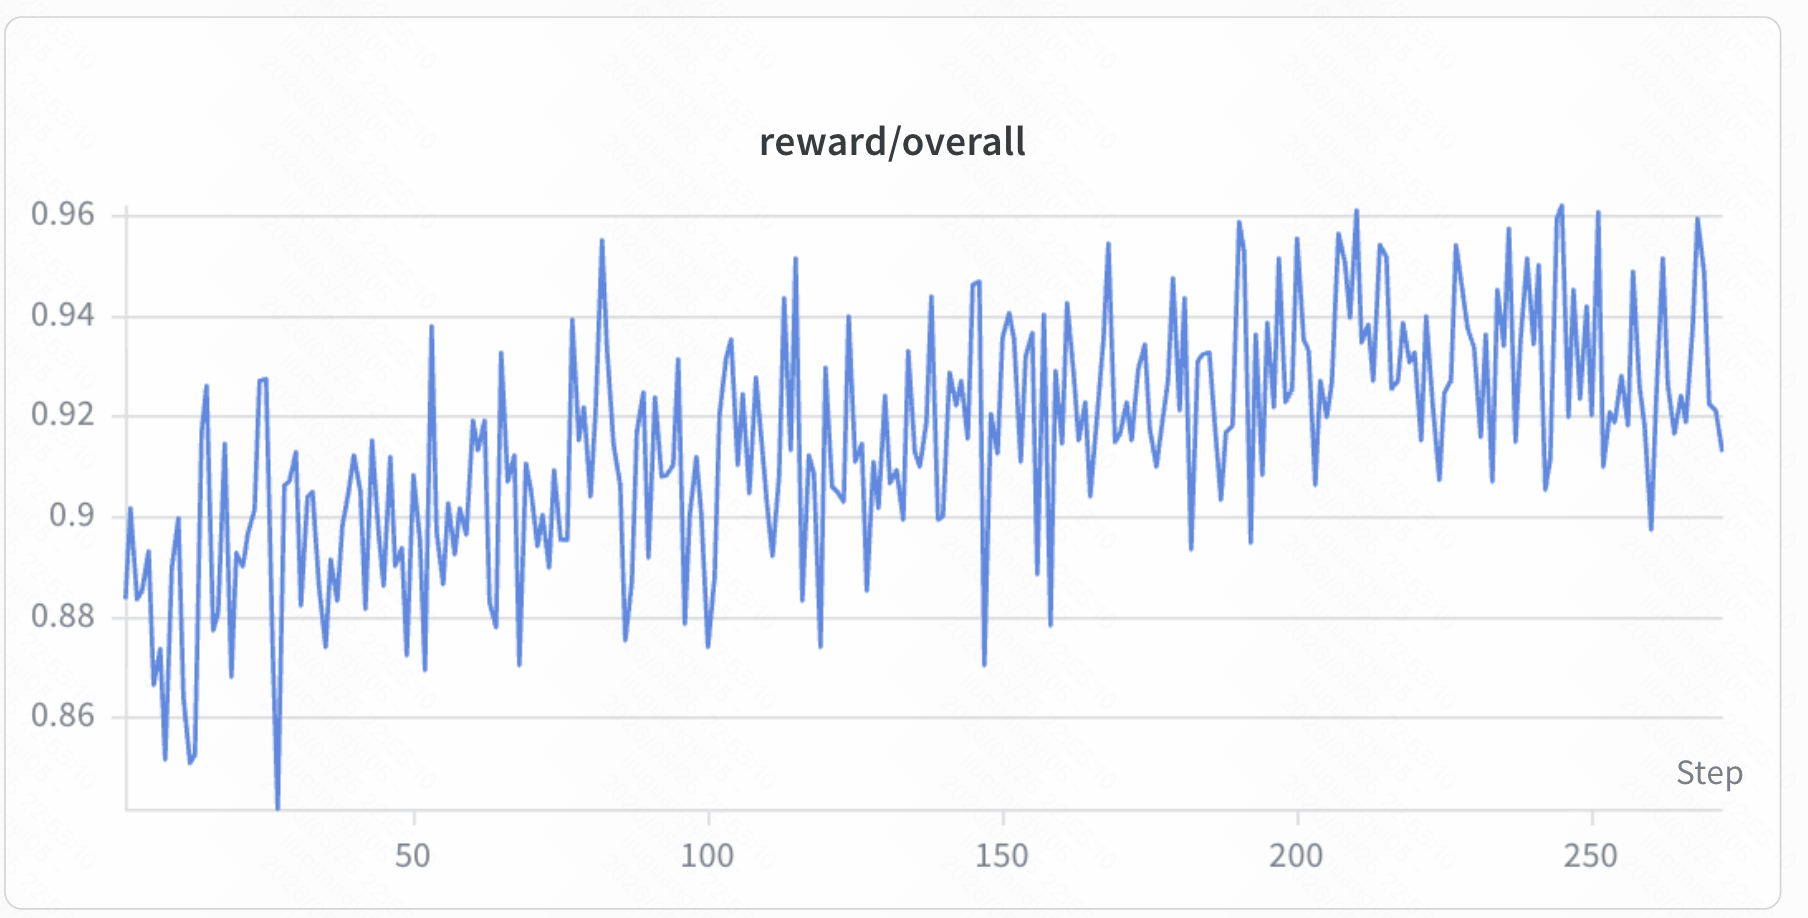
\includegraphics[width=\linewidth]{images/training-curves/qwen3vl-8b-training-900-tasks-reward-overall.png}
  \caption{\llmname{Qwen3-VL-8B}: overall}
\end{subfigure}
\hfill
\begin{subfigure}{0.32\textwidth}
  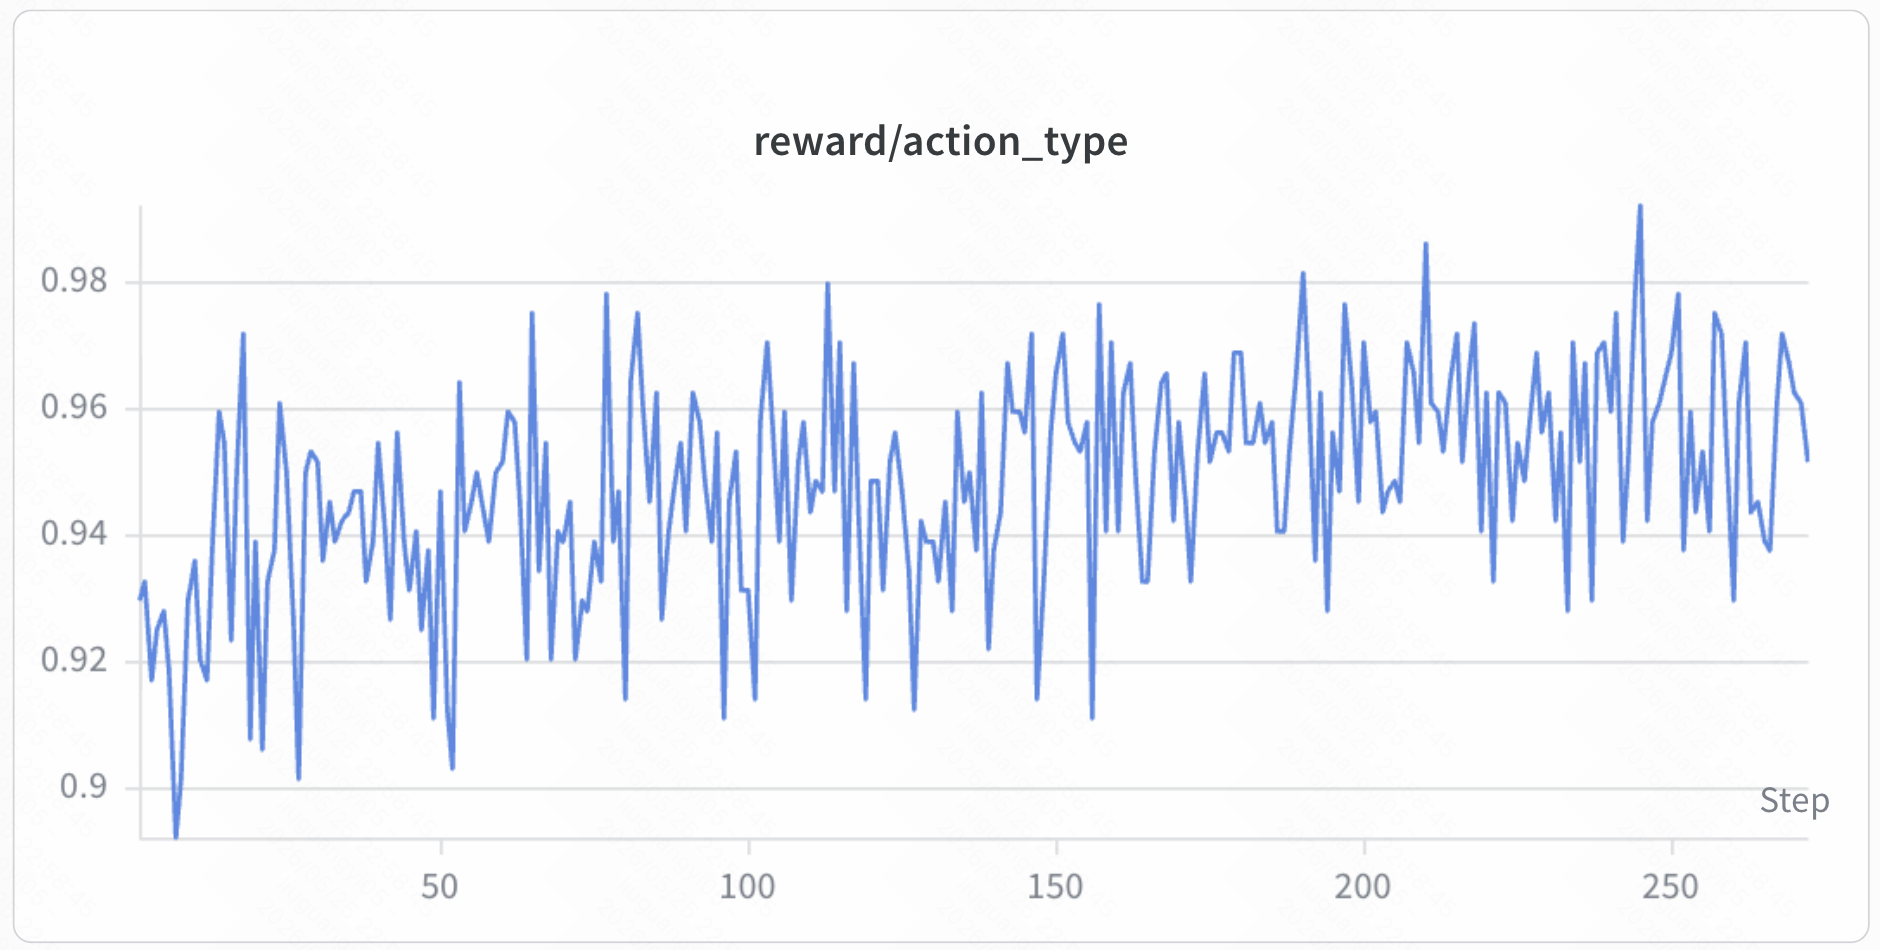
\includegraphics[width=\linewidth]{images/training-curves/qwen3-vl-8b-training-900-tasks-reward-action_type.png}
  \caption{\llmname{Qwen3-VL-8B}: action type}
\end{subfigure}
\hfill
\begin{subfigure}{0.32\textwidth}
  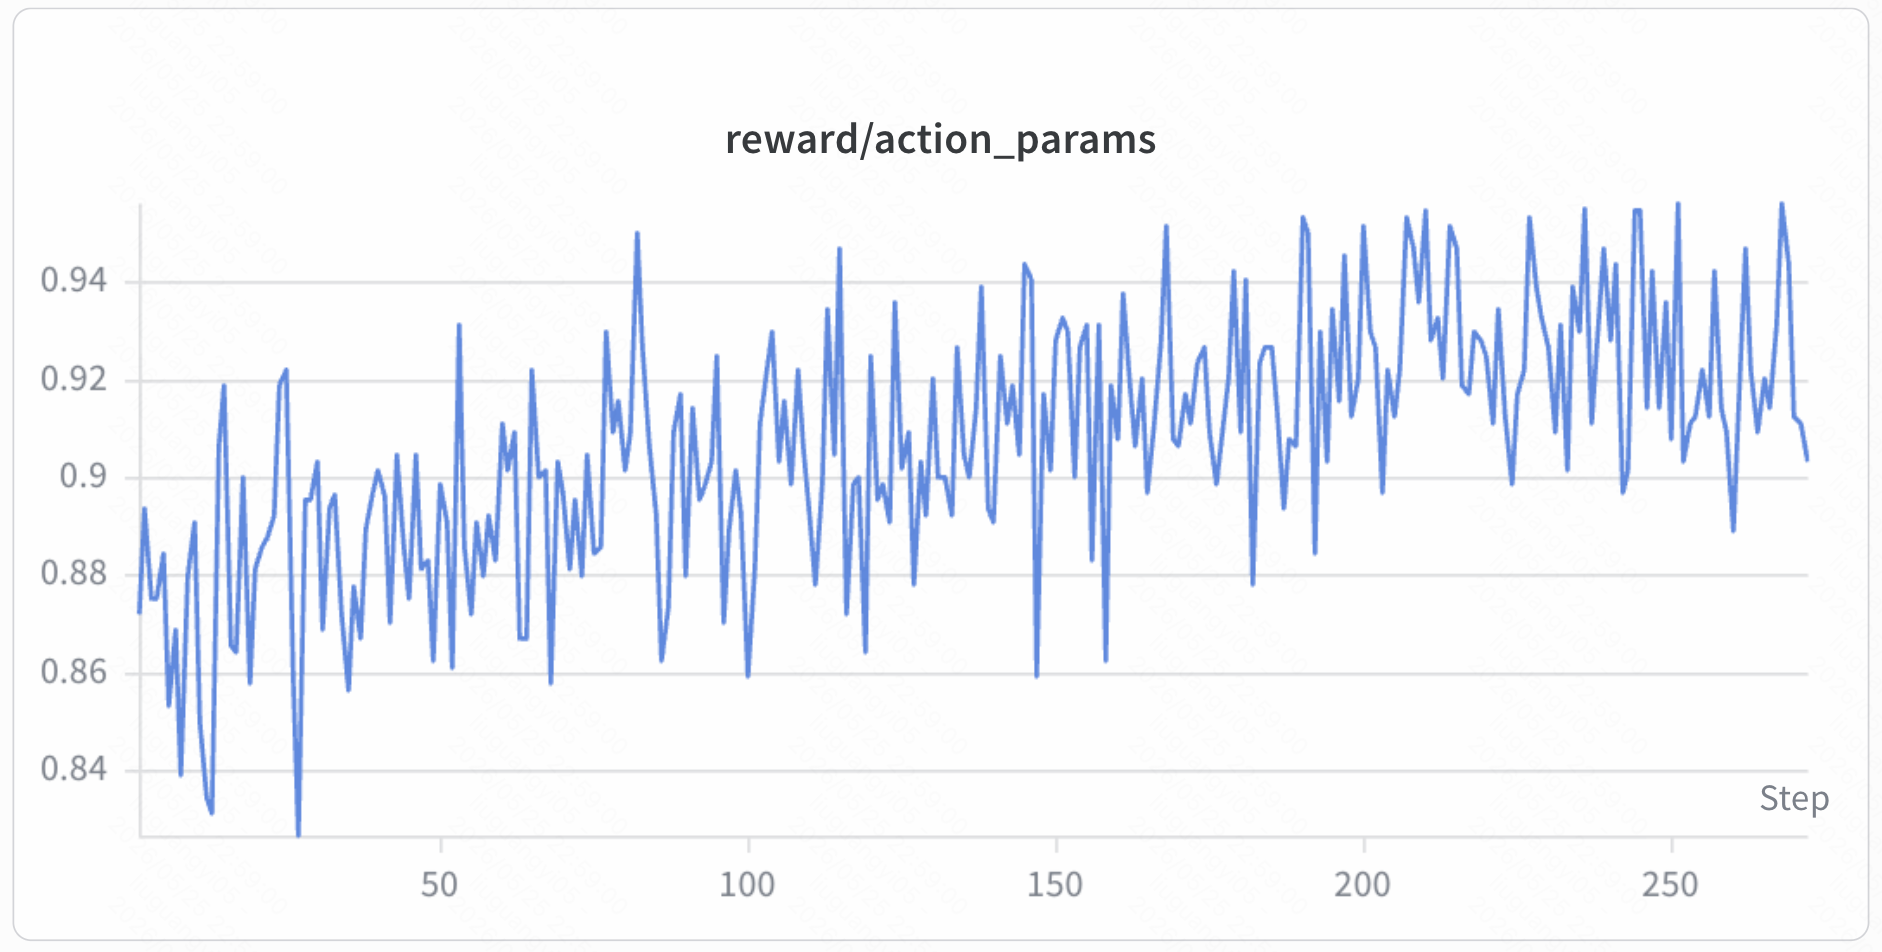
\includegraphics[width=\linewidth]{images/training-curves/qwen3-vl-8b-training-900-tasks-reward-action_params.png}
  \caption{\llmname{Qwen3-VL-8B}: arguments}
\end{subfigure}

\vspace{2mm}
\begin{subfigure}{0.32\textwidth}
  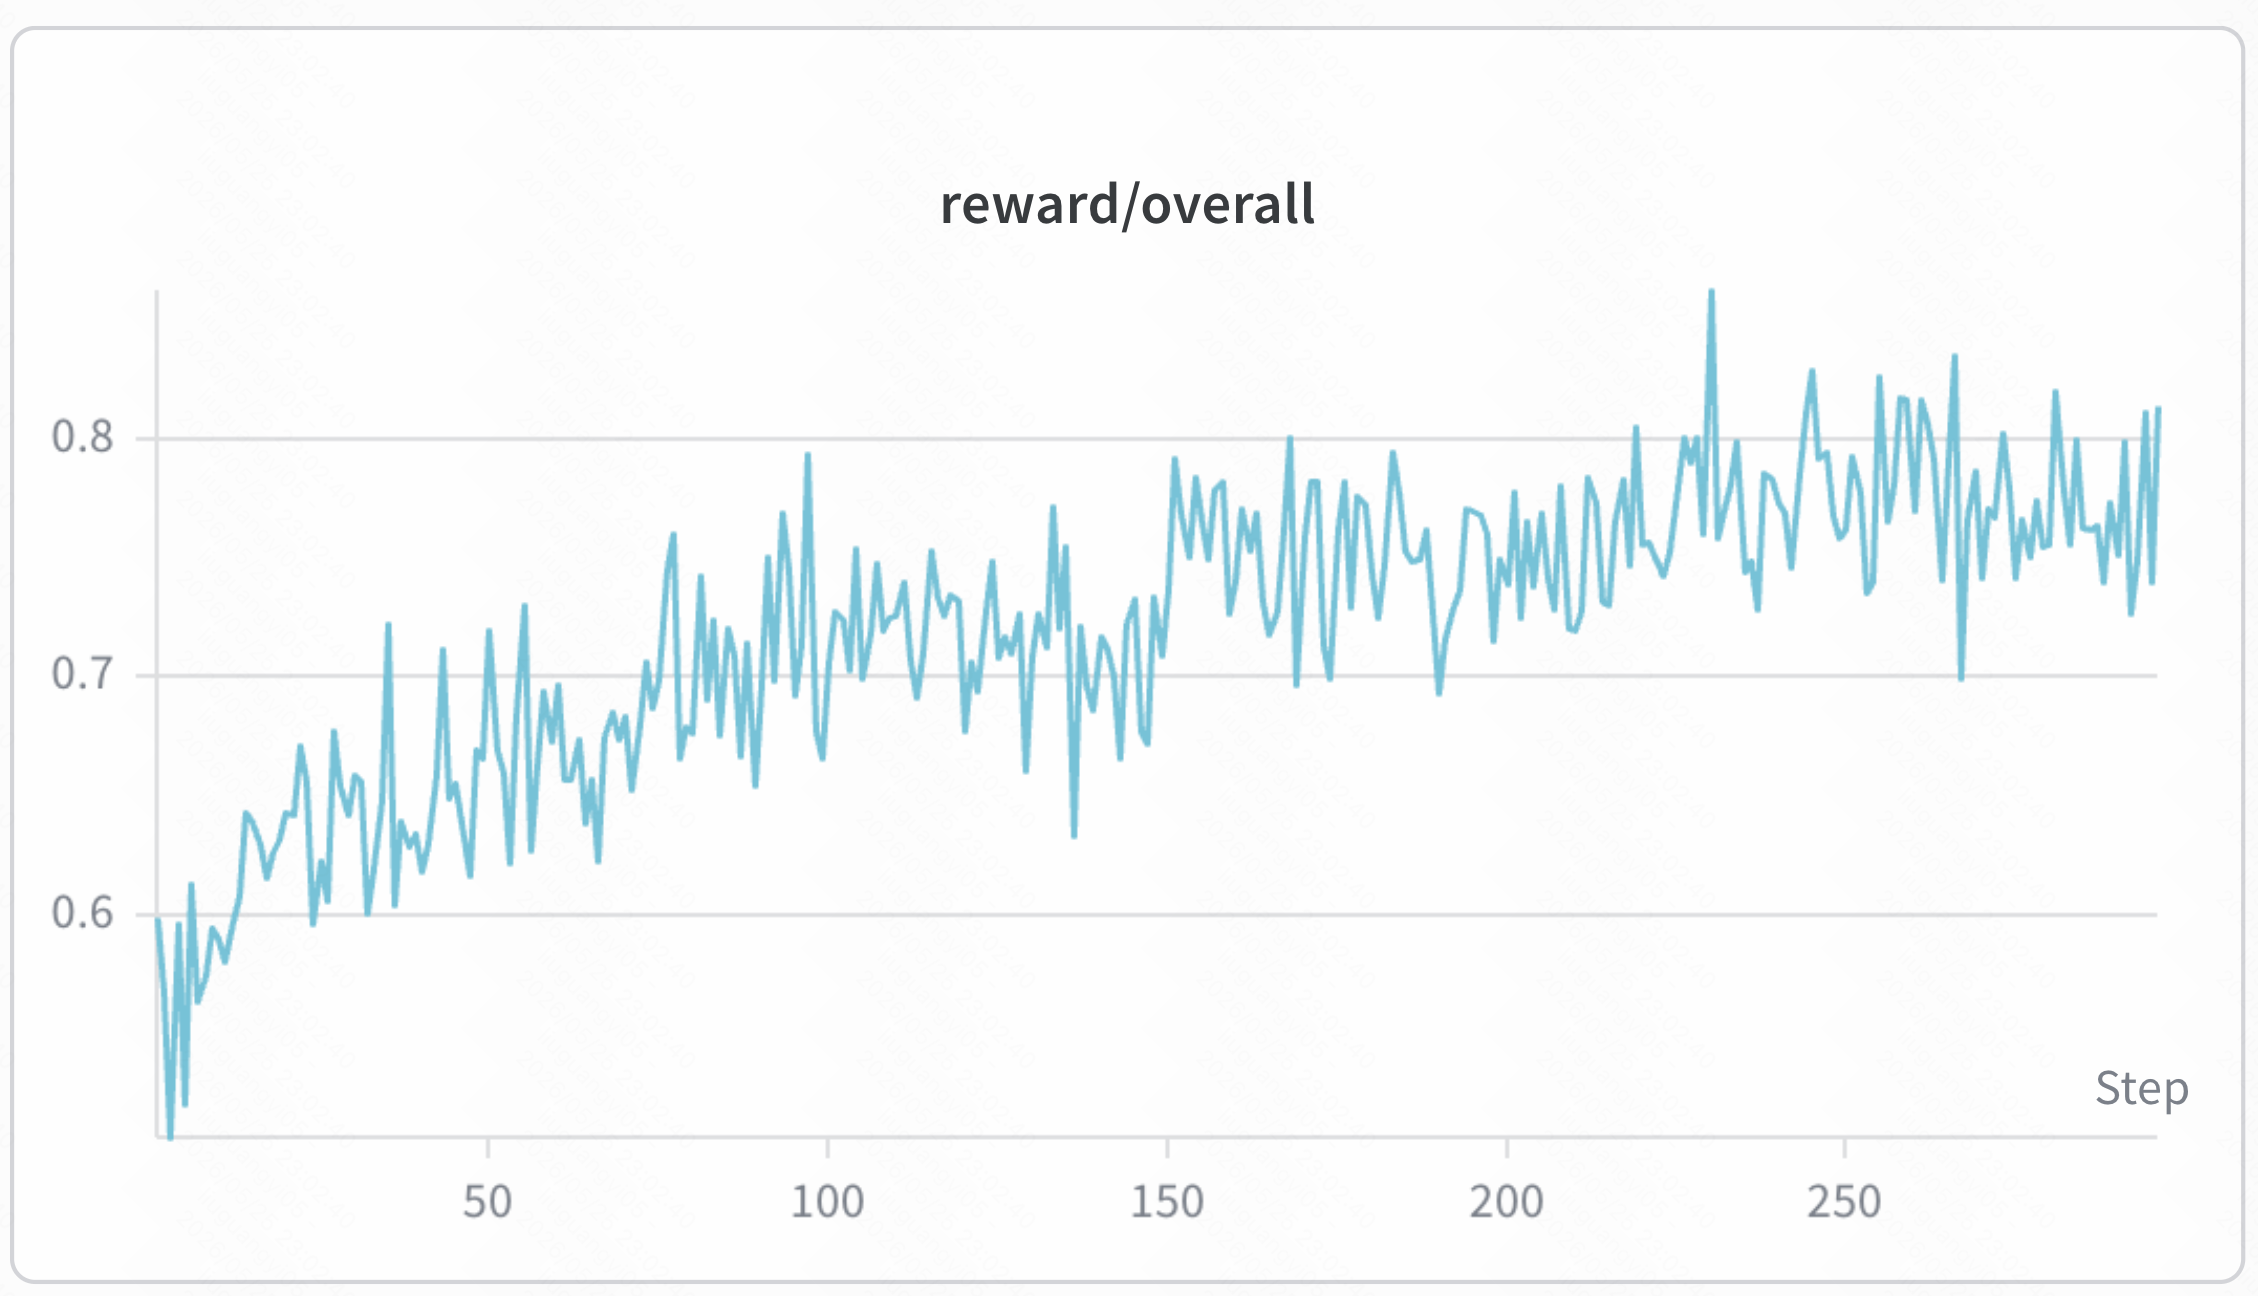
\includegraphics[width=\linewidth]{images/training-curves/gui-owl-1.5-8b-training-900-tasks-reward-overall.png}
  \caption{\llmname{GUI-Owl-1.5-8B}: overall}
\end{subfigure}
\hfill
\begin{subfigure}{0.32\textwidth}
  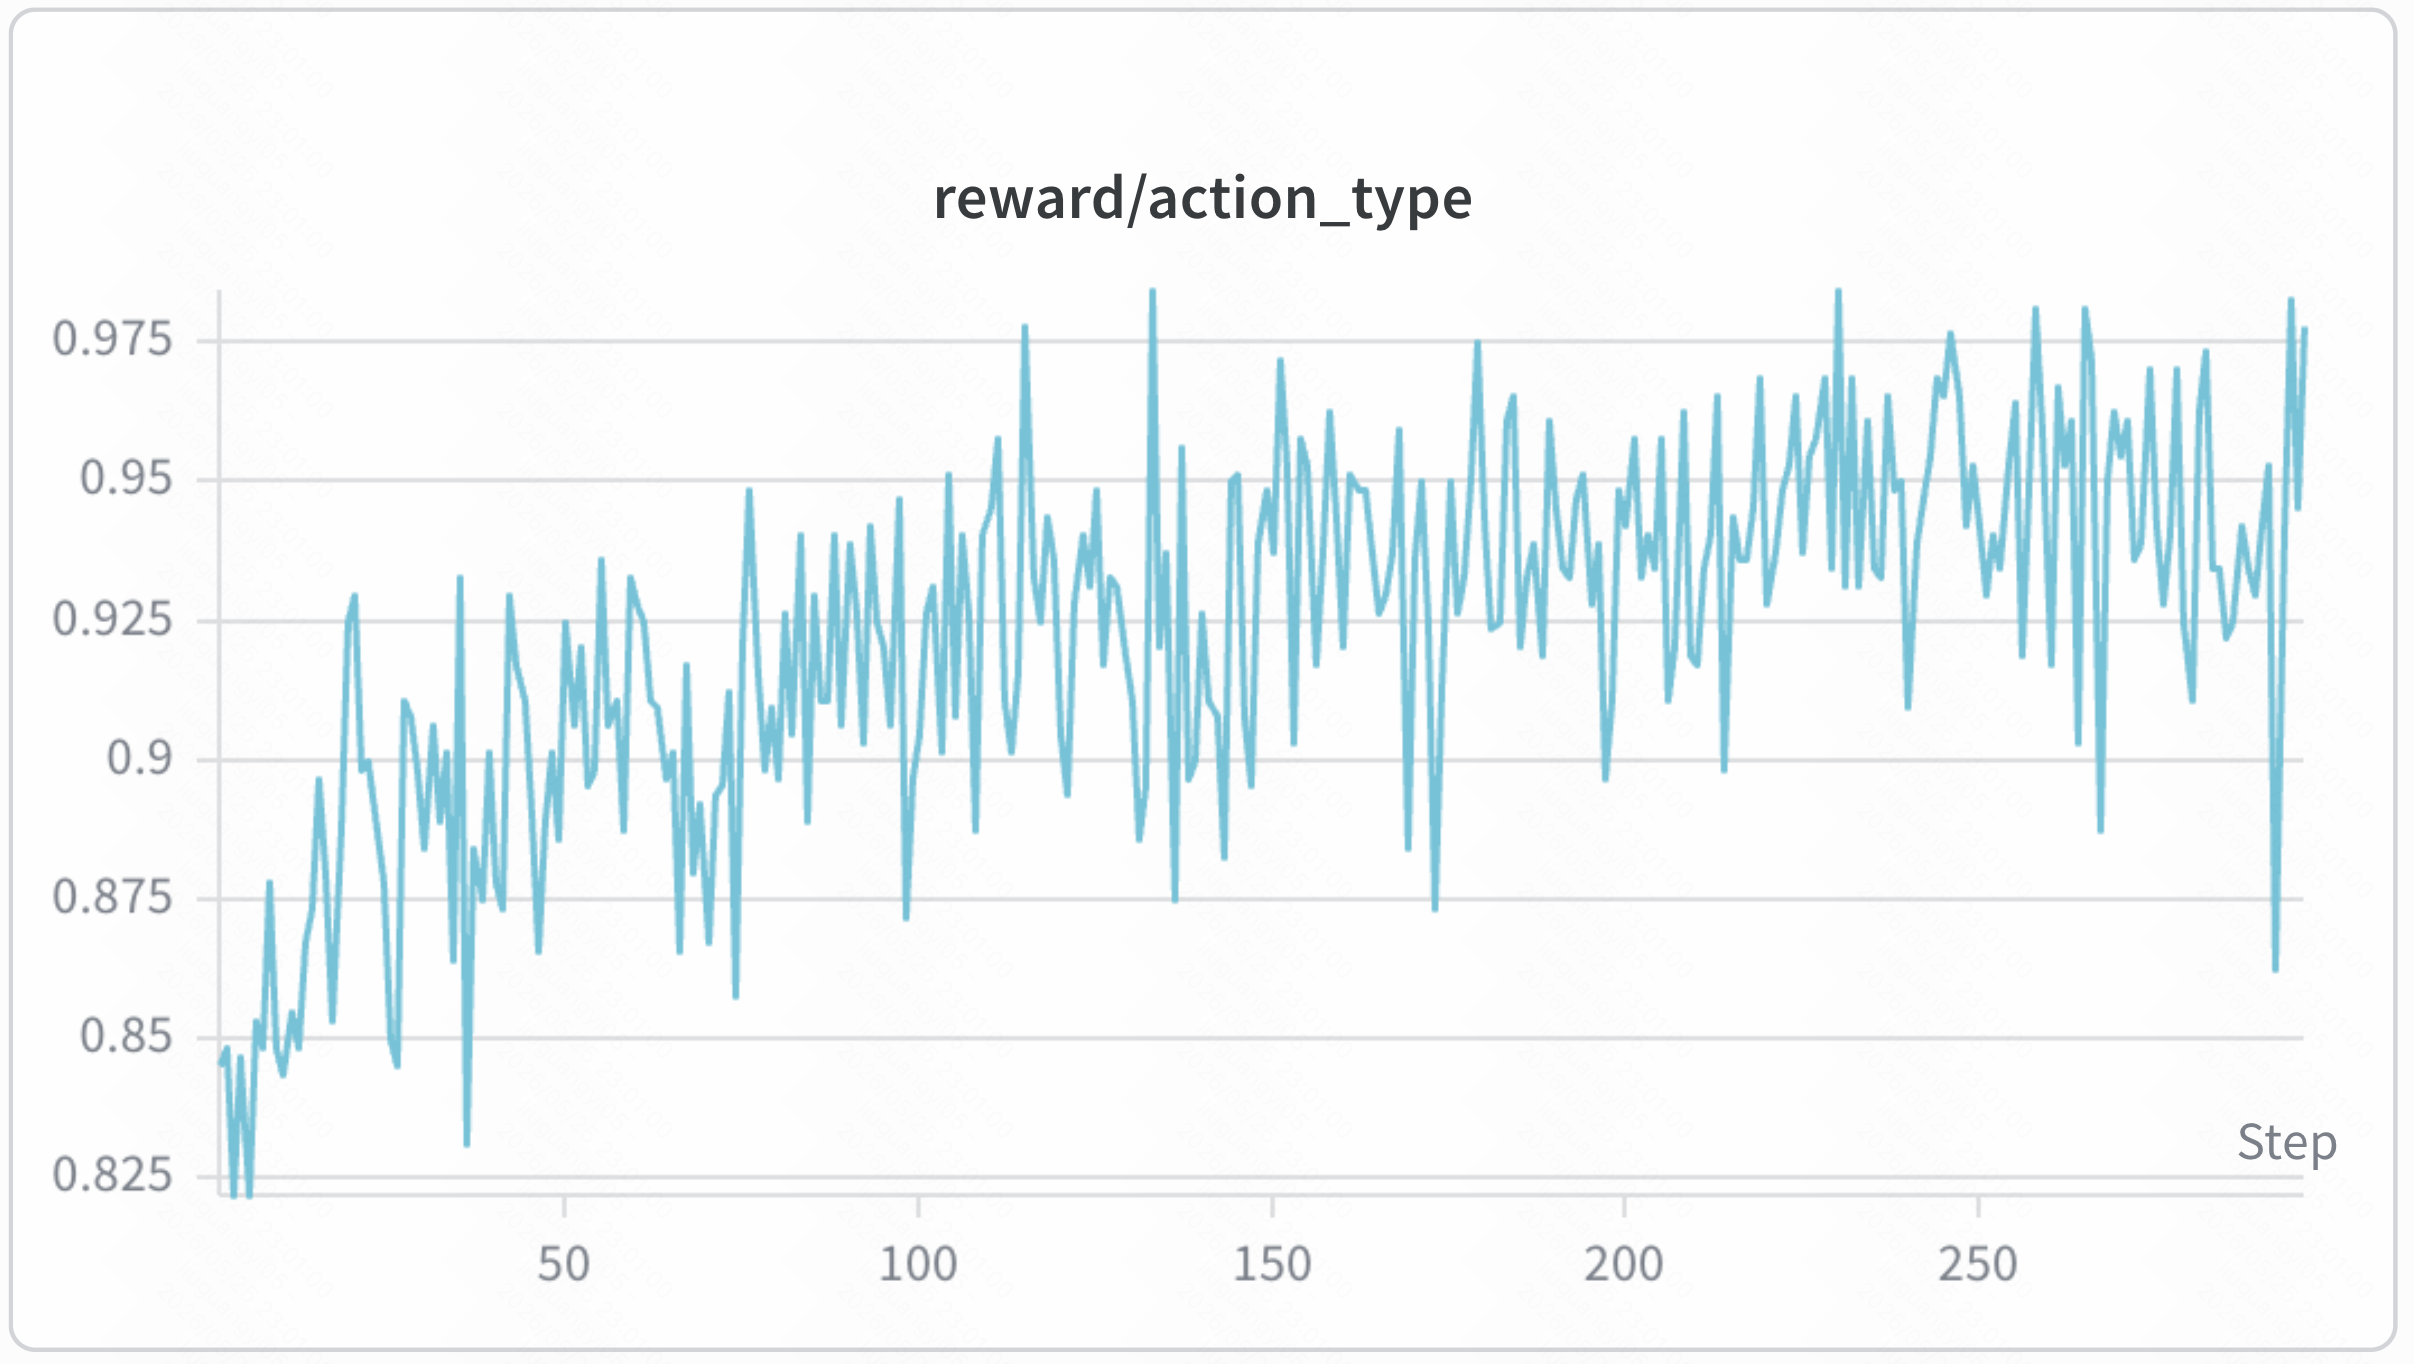
\includegraphics[width=\linewidth]{images/training-curves/gui-owl-1.5-8b-training-900-tasks-reward-action_type.png}
  \caption{\llmname{GUI-Owl-1.5-8B}: action type}
\end{subfigure}
\hfill
\begin{subfigure}{0.32\textwidth}
  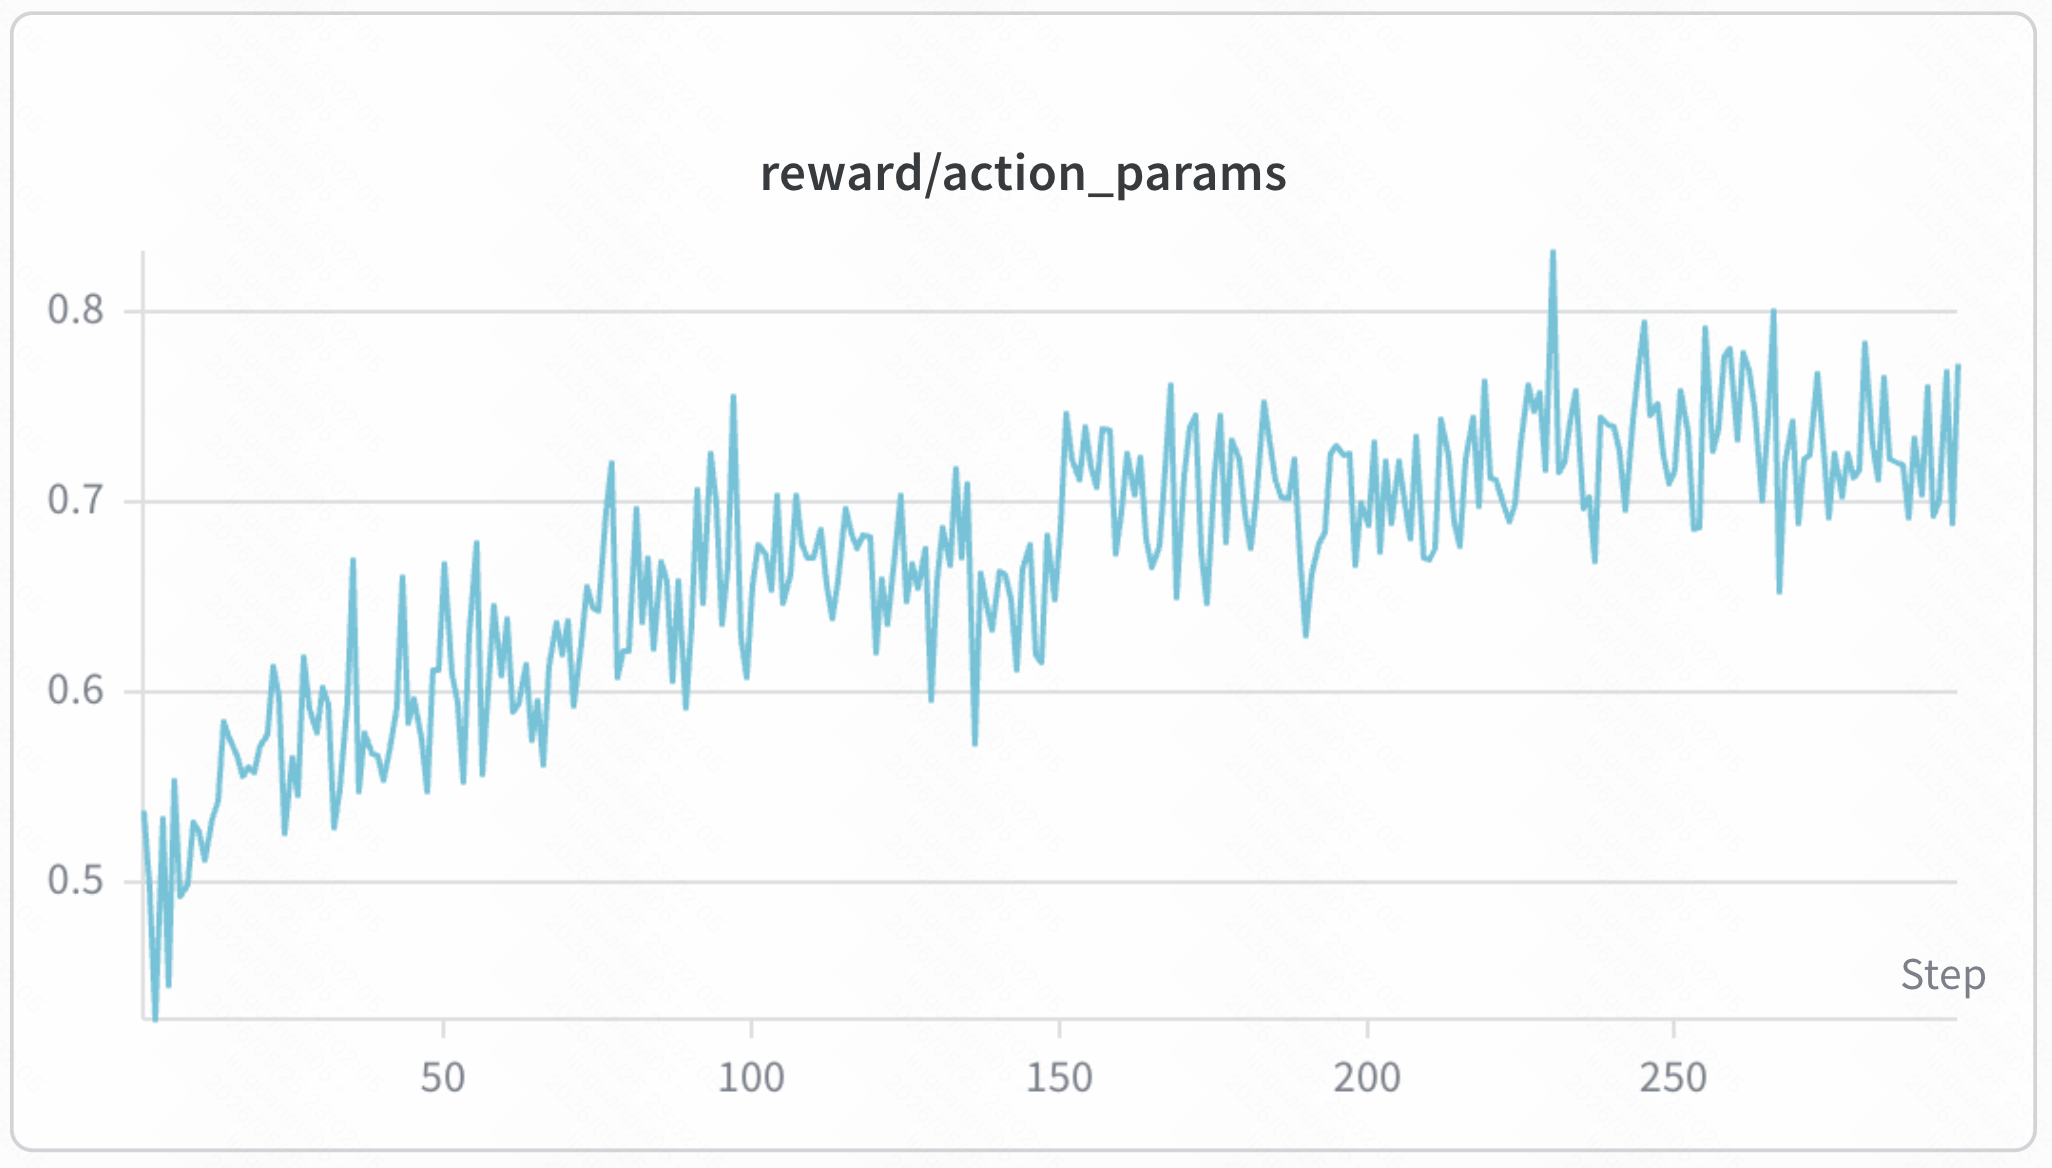
\includegraphics[width=\linewidth]{images/training-curves/gui-owl-1.5-8b-training-900-tasks-reward-action_params.png}
  \caption{\llmname{GUI-Owl-1.5-8B}: arguments}
\end{subfigure}
\caption{Training reward curves for the 900-task \hifpo runs. The overall reward combines action type and action arguments with weights 0.2 and 0.8.}
\label{fig:training_curves}
\end{figure*}

\paragraph{Track-completion cases.}
\label{sec:appendix_track_completion_cases}
Figures~\ref{fig:track_completion_androidworld_qwen}, \ref{fig:track_completion_mobileworld_qwen}, and~\ref{fig:track_completion_mobileworld_guiowl} provide paired base-versus-adapted trajectory comparisons on the same tasks. The examples complement the case study in Section~\ref{sec:case_study_error_analysis} by showing how adaptation changes full task-completion behavior across both AndroidWorld and MobileWorld.



\begin{figure*}[!p]
\centering
\begin{subfigure}[t]{0.49\textwidth}
  \centering
  \includegraphics[width=\linewidth,height=0.68\textheight,keepaspectratio]{images/track-completion-comparison/AndroidWorld-qwen-base.png}
  \caption{\llmname{Qwen3-VL-8B} base: failed}
\end{subfigure}
\hfill
\begin{subfigure}[t]{0.49\textwidth}
  \centering
  \includegraphics[width=\linewidth,height=0.68\textheight,keepaspectratio]{images/track-completion-comparison/AndroidWorld-qwen-rl.png}
  \caption{\llmname{ForgeQwen3-8B}: successful}
\end{subfigure}
\caption{\textbf{AndroidWorld track-completion comparison for \llmname{Qwen3-VL-8B}.}
On the same Broccoli recipe-deletion task, the base model falls into repeated scrolling after partial progress, while \ourmethod adaptation enables \llmname{ForgeQwen3-8B} to switch to a targeted search strategy and complete the remaining deletion.}
\label{fig:track_completion_androidworld_qwen}
\end{figure*}

\begin{figure*}[!p]
\centering
\begin{subfigure}[t]{0.49\textwidth}
  \centering
  \includegraphics[width=\linewidth,height=0.68\textheight,keepaspectratio]{images/track-completion-comparison/MobileWorld-qwen-base.png}
  \caption{\llmname{Qwen3-VL-8B} base: failed}
\end{subfigure}
\hfill
\begin{subfigure}[t]{0.49\textwidth}
  \centering
  \includegraphics[width=\linewidth,height=0.68\textheight,keepaspectratio]{images/track-completion-comparison/MobileWorld-qwen-rl.png}
  \caption{\llmname{ForgeQwen3-8B}: successful}
\end{subfigure}
\caption{\textbf{MobileWorld track-completion comparison for \llmname{Qwen3-VL-8B}.}
On the same multi-app academic-calendar and email task, the base model selects an underspecified semester result and then skips the calendar subtask, while \llmname{ForgeQwen3-8B} verifies the Spring 2026 deadline window, creates the calendar event, and proceeds to the email workflow.}
\label{fig:track_completion_mobileworld_qwen}
\end{figure*}

\begin{figure*}[!p]
\centering
\begin{subfigure}[t]{0.49\textwidth}
  \centering
  \includegraphics[width=\linewidth,height=0.68\textheight,keepaspectratio]{images/track-completion-comparison/MobileWorld-guiowl-base.png}
  \caption{\llmname{GUI-Owl-1.5-8B} base: failed}
\end{subfigure}
\hfill
\begin{subfigure}[t]{0.49\textwidth}
  \centering
  \includegraphics[width=\linewidth,height=0.68\textheight,keepaspectratio]{images/track-completion-comparison/MobileWorld-guiowl-rl.png}
  \caption{\llmname{ForgeOwl-8B}: successful}
\end{subfigure}
\caption{\textbf{MobileWorld track-completion comparison for \llmname{GUI-Owl-1.5-8B}.}
On the same invoice recalculation and email task, the base model leaves the invoice context too early and sends an incorrect amount, while \llmname{ForgeOwl-8B} preserves the key invoice conditions, shares the document into Mail, and sends the correct recalculated total.}
\label{fig:track_completion_mobileworld_guiowl}
\end{figure*}
\end{document}
